% !TeX program = xelatex
\documentclass[a4paper,10pt]{article}

% ============================================================================
% កញ្ចប់សម្ភារៈសិក្សាបោះពុម្ព ស-ខ្មៅ (Printable Classroom Materials - Grade 8 SAS)
% ត្រូវគ្នា ១០០% នឹង LS_Plan_SAS.tex និង Teaching_Scenario_SAS.tex
% ============================================================================
\usepackage[a4paper, left=1.0cm, right=1.0cm, top=0.75cm, bottom=1.05cm, footskip=0.55cm]{geometry}
\usepackage{amsmath, amssymb}
\usepackage{unicode-math}
\usepackage{fontspec}
\usepackage{array, colortbl}
\usepackage[table]{xcolor}
\usepackage{enumitem}
\usepackage{pifont}
\usepackage{fancyhdr}
\usepackage{lastpage}
\usepackage{tikz}
\usepackage[most]{tcolorbox}
\usetikzlibrary{calc, arrows.meta, angles, quotes, decorations.markings, babel}

% LaTeX 2025 compatibility guard
\makeatletter
\let\@expl@@@mark@update@singlecol@structures@@\relax
\makeatother

% ============================================================================
% ការកំណត់ពុម្ពអក្សរផ្លូវការ (Word-Styled Khmer + Cambria Math + Times New Roman)
% ============================================================================
% Cross-platform font path resolver (Windows local + Linux/Cloud repo fonts/)
\providecommand{\NGSFindFonts}{%
  \IfFileExists{C:/Windows/Fonts/cambria.ttc}{%
    \def\NGSSysPath{C:/Windows/Fonts/}%
    \def\NGSUserPath{C:/Users/KIT/AppData/Local/Microsoft/Windows/Fonts/}%
  }{%
    \IfFileExists{./fonts/KhmerOSsiemreap.ttf}{\def\NGSSysPath{./fonts/}\def\NGSUserPath{./fonts/}}{%
    \IfFileExists{../fonts/KhmerOSsiemreap.ttf}{\def\NGSSysPath{../fonts/}\def\NGSUserPath{../fonts/}}{%
    \IfFileExists{../../fonts/KhmerOSsiemreap.ttf}{\def\NGSSysPath{../../fonts/}\def\NGSUserPath{../../fonts/}}{%
    \IfFileExists{../../../fonts/KhmerOSsiemreap.ttf}{\def\NGSSysPath{../../../fonts/}\def\NGSUserPath{../../../fonts/}}{%
    \IfFileExists{../../../../fonts/KhmerOSsiemreap.ttf}{\def\NGSSysPath{../../../../fonts/}\def\NGSUserPath{../../../../fonts/}}{%
    \IfFileExists{../../../../../fonts/KhmerOSsiemreap.ttf}{\def\NGSSysPath{../../../../../fonts/}\def\NGSUserPath{../../../../../fonts/}}{%
    \IfFileExists{../../../../../../fonts/KhmerOSsiemreap.ttf}{\def\NGSSysPath{../../../../../../fonts/}\def\NGSUserPath{../../../../../../fonts/}}{%
      \def\NGSSysPath{../../../../../../../fonts/}\def\NGSUserPath{../../../../../../../fonts/}%
    }}}}}}}%
  }%
}
\NGSFindFonts

\setmathfont[
  Path={\NGSSysPath},
  FontIndex=1,
  Scale=1.02
]{cambria.ttc}

\defaultfontfeatures{Ligatures=TeX}

\setmainfont[
  Path={\NGSUserPath},
  Extension=.ttf,
  Script=Khmer,
  BoldFont={KhmerOSsiemreap},
  BoldFeatures={FakeBold=1.8},
  ItalicFont={KhmerOSsiemreap},
  ItalicFeatures={FakeSlant=0.25},
  BoldItalicFont={KhmerOSsiemreap},
  BoldItalicFeatures={FakeBold=1.8, FakeSlant=0.25}
]{KhmerOSsiemreap}

\newfontfamily\muol[
  Path={\NGSUserPath},
  Extension=.ttf,
  Script=Khmer
]{KhmerOSmuollight}

\newfontfamily\TimesEn[
  Path={\NGSSysPath},
  Extension=.ttf,
  BoldFont={timesbd},
  ItalicFont={timesi},
  BoldItalicFont={timesbi}
]{times}

\newfontfamily\CalibriFont[
  Path={\NGSSysPath},
  Extension=.ttf
]{calibri}

\newfontfamily\Tacteing[
  Path={\NGSUserPath}
]{TACTENG.TTF}

\XeTeXlinebreaklocale "km"
\XeTeXlinebreakskip = 0pt plus 1pt minus 0.1pt

% ============================================================================
% ក្ដារពណ៌ ស-ខ្មៅ សុទ្ធសម្រាប់ការបោះពុម្ព (Strict Monochrome Print Palette)
% ============================================================================
\definecolor{panelgray}{gray}{0.92} % ~gray!8
\definecolor{headgray}{gray}{0.85}  % ~gray!15
\definecolor{midgray}{gray}{0.75}   % ~gray!25
\definecolor{darkline}{gray}{0.35}  % ~gray!65

\pagestyle{fancy}
\fancyhf{}
\renewcommand{\headrulewidth}{0pt}
\fancyfoot[L]{\fontsize{8pt}{10pt}\selectfont អនុវិទ្យាល័យព្រះក្រសាំង — គណិតវិទ្យា ថ្នាក់ទី៨ | មេរៀនទី១២ (១.២.២) ករណី \en{SAS} (ស-ខ្មៅ)}
\fancyfoot[R]{\fontsize{8.5pt}{10pt}\selectfont ទំព័រ \en{\thepage\ / \pageref{LastPage}}}

\setlength{\parindent}{0pt}
\setlength{\parskip}{0pt}
\setlength{\tabcolsep}{4pt}

% ============================================================================
% ម៉ាក្រូជំនួយ (Helper Macros)
% ============================================================================
\newcommand{\en}[1]{{\TimesEn #1}}
\newcommand{\unit}[1]{\,\text{\en{#1}}}
\newcommand{\cnum}[1]{{\fontsize{10pt}{12pt}\selectfont\ding{\numexpr181+#1\relax}}}
\newcommand{\scissors}{\ding{34}}
\newcommand{\chkbox}{\tikz[baseline=-0.15ex]\draw[black, line width=0.85pt] (0,0) rectangle (0.26cm,0.26cm);}
\newcommand{\tickone}{\tikz[baseline=-0.2ex]\draw[black, line width=1.1pt] (0,0) -- (0,0.25cm);}
\newcommand{\ticktwo}{\tikz[baseline=-0.2ex]{\draw[black, line width=1.1pt] (0,0) -- (0,0.25cm);\draw[black, line width=1.1pt] (0.08cm,0) -- (0.08cm,0.25cm);}}
\newcommand{\tri}[1]{\ensuremath{\triangle #1}}
\newcommand{\ang}[1]{\ensuremath{\angle #1}}
\newcommand{\cg}{\ensuremath{\cong}}
\newcommand{\ncg}{\ensuremath{\not\cong}}
\newcommand{\khmflourish}{{\Tacteing\fontsize{32pt}{12pt}\selectfont\raisebox{-4pt}{3}}}

\newcommand{\pagebanner}[2]{%
  \begin{tcolorbox}[
    enhanced, sharp corners, colback=headgray, colframe=black,
    boxrule=1.1pt, top=3pt, bottom=3pt, left=6pt, right=6pt,
    after skip=4pt
  ]
    {\muol\fontsize{10.5pt}{15pt}\selectfont #1}\hfill{\fontsize{8.5pt}{12pt}\selectfont\textbf{#2}}
  \end{tcolorbox}%
}

\newcolumntype{L}[1]{>{\raggedright\arraybackslash}p{#1}}
\newcolumntype{C}[1]{>{\centering\arraybackslash}p{#1}}

% Bold B&W Tick marks (>=1.0pt print safe)
\tikzset{
  tk1/.style={postaction={decorate},decoration={markings,
    mark=at position 0.50 with {\draw[black, line width=1.05pt] (0,-0.11)--(0,0.11);}}},
  tk2/.style={postaction={decorate},decoration={markings,
    mark=at position 0.44 with {\draw[black, line width=1.05pt] (0,-0.11)--(0,0.11);},
    mark=at position 0.56 with {\draw[black, line width=1.05pt] (0,-0.11)--(0,0.11);}}}
}

\begin{document}
\fontsize{9.2pt}{13.5pt}\selectfont

% ============================================================================
% ទំព័រទី ១៖ បន្ទះចង្កឹះបត់គន្លឹះ E2 ខ្នាតពិត 1:1 & ផ្ទាំងពិសោធន៍ POE 32°
% ============================================================================
\pagebanner{សម្ភារៈទី ១៖ បន្ទះចង្កឹះបត់គន្លឹះ \en{E2} ខ្នាតពិត \en{1:1} និងផ្ទាំង \en{POE} មុំ $32^\circ$}{ទំព័រទី ១ / ៦ — សកម្មភាព \en{E2 Explore}}

% --- ប្រអប់ព្រមានខ្នាតពិត & បន្ទះផ្ទៀង 5 cm (x=1cm, y=1cm) ---
\noindent
\begin{minipage}[c]{11.9cm}
  \begin{tcolorbox}[
    enhanced, sharp corners, colback=panelgray, colframe=black,
    boxrule=1.0pt, top=3.5pt, bottom=3.5pt, left=6pt, right=6pt
  ]
    \fontsize{8.8pt}{12.5pt}\selectfont
    \textbf{ការណែនាំសំខាន់មុនបោះពុម្ព៖} ពេលបោះពុម្ព សូមជ្រើស \textbf{\en{Scale: Actual Size 100\%}} — \textbf{កុំជ្រើស \en{Fit to Page}} ដើម្បីឱ្យបន្ទះ $4\unit{cm}$, $6\unit{cm}$, $5\unit{cm}$ និងមុំ $32^\circ$ វាស់ត្រូវពិតប្រាកដតាមបន្ទាត់ និងរ៉ាប៉ទ័រ។\\[2pt]
    \textbf{វិធីរៀបចំសិស្ស៖} កាត់បន្ទះតាមស្នាមចុច \scissors{} ហើយចោះរន្ធតូចត្រង់សញ្ញា \textbf{\en{o}} ដោយម្ជុលខ្ទាស់ ឬក្រដាសកាត់ផ្ទៀង។
  \end{tcolorbox}
\end{minipage}%
\hfill
\begin{minipage}[c]{6.8cm}
  \begin{tcolorbox}[
    enhanced, sharp corners, colback=white, colframe=black,
    boxrule=1.0pt, top=3pt, bottom=3pt, left=4pt, right=4pt
  ]
    \centering
    {\fontsize{8.2pt}{11pt}\selectfont\textbf{បន្ទះផ្ទៀងខ្នាតពិត \en{5 cm} (\en{1:1 Ruler Check})}}\\[2pt]
    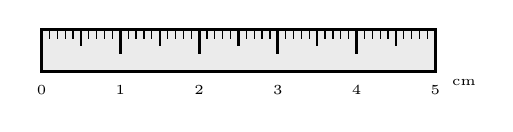
\begin{tikzpicture}[x=1cm, y=1cm, every node/.style={font=\scriptsize, text=black}]
      \draw[black, line width=1.1pt, fill=panelgray] (0,0) rectangle (5.0, 0.54);
      \foreach \m in {0,...,50}{
        \pgfmathsetmacro{\xval}{\m*0.1}
        \draw[black, line width=0.45pt] (\xval, 0.54) -- (\xval, 0.41);
      }
      \foreach \h in {0,0.5,...,5.0}{
        \draw[black, line width=0.8pt] (\h, 0.54) -- (\h, 0.33);
      }
      \foreach \c in {0,1,2,3,4,5}{
        \draw[black, line width=1.1pt] (\c, 0.54) -- (\c, 0.22);
        \node[below=1.2pt, font=\tiny] at (\c, 0.0) {\en{\c}};
      }
      \node[right=2pt, font=\tiny] at (5.02, -0.14) {\en{cm}};
    \end{tikzpicture}
  \end{tcolorbox}
\end{minipage}

\vspace{4pt}

% --- ផ្នែកទី ១៖ បន្ទះគន្លឹះកាត់តាមស្នាមចុច 4cm, 6cm, 5cm (x=1cm, y=1cm, ZERO scaling) ---
\textbf{១. បន្ទះចង្កឹះគន្លឹះកាត់តាមស្នាមចុច \scissors{} (ខ្នាតពិត \en{x=1cm, y=1cm} — ចម្ងាយរវាងចំណុចកណ្ដាលរន្ធ \en{o} ទាំងពីរ)}

\vspace{2pt}
\begin{center}
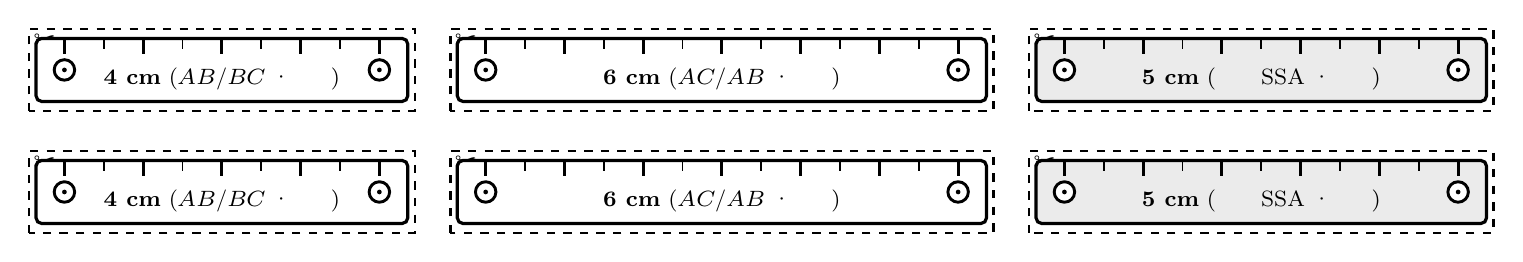
\begin{tikzpicture}[x=1cm, y=1cm, every node/.style={font=\scriptsize, text=black}]
  % ឈុតទី ១ (Row 1) និង ឈុតទី ២ (Row 2)
  \foreach \row/\yoff/\lbl in {1/1.55/ឈុត ១, 2/0.0/ឈុត ២}{
    % --- បន្ទះ 4 cm (pin-to-pin exact 4.0 cm) ---
    \begin{scope}[shift={(0.45, \yoff)}]
      \draw[black, dashed, line width=0.95pt] (-0.45, -0.52) rectangle (4.45, 0.52);
      \node[anchor=north west, inner sep=1pt, font=\footnotesize] at (-0.43, 0.50) {\scissors};
      \draw[black, line width=1.15pt, rounded corners=2pt, fill=white] (-0.36, -0.40) rectangle (4.36, 0.40);
      \foreach \h in {0,0.5,...,4.0}{
        \draw[black, line width=0.65pt] (\h, 0.40) -- (\h, 0.27);
      }
      \foreach \k in {0,1,2,3,4}{
        \draw[black, line width=1.05pt] (\k, 0.40) -- (\k, 0.20);
      }
      \draw[black, line width=1.05pt, fill=white] (0,0) circle (0.13);
      \fill[black] (0,0) circle (0.03);
      \draw[black, line width=1.05pt, fill=white] (4,0) circle (0.13);
      \fill[black] (4,0) circle (0.03);
      \node[font=\footnotesize] at (2.0, -0.11) {\textbf{\en{4 cm}} ($AB/BC$ · \lbl)};
    \end{scope}

    % --- បន្ទះ 6 cm (pin-to-pin exact 6.0 cm) ---
    \begin{scope}[shift={(5.80, \yoff)}]
      \draw[black, dashed, line width=0.95pt] (-0.45, -0.52) rectangle (6.45, 0.52);
      \node[anchor=north west, inner sep=1pt, font=\footnotesize] at (-0.43, 0.50) {\scissors};
      \draw[black, line width=1.15pt, rounded corners=2pt, fill=white] (-0.36, -0.40) rectangle (6.36, 0.40);
      \foreach \h in {0,0.5,...,6.0}{
        \draw[black, line width=0.65pt] (\h, 0.40) -- (\h, 0.27);
      }
      \foreach \k in {0,1,2,3,4,5,6}{
        \draw[black, line width=1.05pt] (\k, 0.40) -- (\k, 0.20);
      }
      \draw[black, line width=1.05pt, fill=white] (0,0) circle (0.13);
      \fill[black] (0,0) circle (0.03);
      \draw[black, line width=1.05pt, fill=white] (6,0) circle (0.13);
      \fill[black] (6,0) circle (0.03);
      \node[font=\footnotesize] at (3.0, -0.11) {\textbf{\en{6 cm}} ($AC/AB$ · \lbl)};
    \end{scope}

    % --- បន្ទះបញ្ឆោត 5 cm (pin-to-pin exact 5.0 cm) ---
    \begin{scope}[shift={(13.15, \yoff)}]
      \draw[black, dashed, line width=0.95pt] (-0.45, -0.52) rectangle (5.45, 0.52);
      \node[anchor=north west, inner sep=1pt, font=\footnotesize] at (-0.43, 0.50) {\scissors};
      \draw[black, line width=1.15pt, rounded corners=2pt, fill=panelgray] (-0.36, -0.40) rectangle (5.36, 0.40);
      \foreach \h in {0,0.5,...,5.0}{
        \draw[black, line width=0.65pt] (\h, 0.40) -- (\h, 0.27);
      }
      \foreach \k in {0,1,2,3,4,5}{
        \draw[black, line width=1.05pt] (\k, 0.40) -- (\k, 0.20);
      }
      \draw[black, line width=1.05pt, fill=white] (0,0) circle (0.13);
      \fill[black] (0,0) circle (0.03);
      \draw[black, line width=1.05pt, fill=white] (5,0) circle (0.13);
      \fill[black] (5,0) circle (0.03);
      \node[font=\footnotesize] at (2.5, -0.11) {\textbf{\en{5 cm}} (បញ្ឆោត \en{SSA} · \lbl)};
    \end{scope}
  }
\end{tikzpicture}
\end{center}

\vspace{2pt}

% --- ផ្នែកទី ២៖ ផ្ទាំងពិសោធន៍ POE ២ ផ្ទាំង (មុំ 32°, AB = 6 cm, x=1cm, y=1cm) ---
\textbf{២. ផ្ទាំងពិសោធន៍ \en{POE} ប៉ោលដៃផ្ទាល់ មុំ $32^\circ$ ចំនួន ២ ផ្ទាំង (ខ្នាតពិត \en{x=1cm, y=1cm})} — ខ្ទាស់បន្ទះ $4\unit{cm}$ ត្រង់ $B$ រួចយោលកាត់កន្លះបន្ទាត់ $Ax$

\vspace{2pt}
\begin{center}
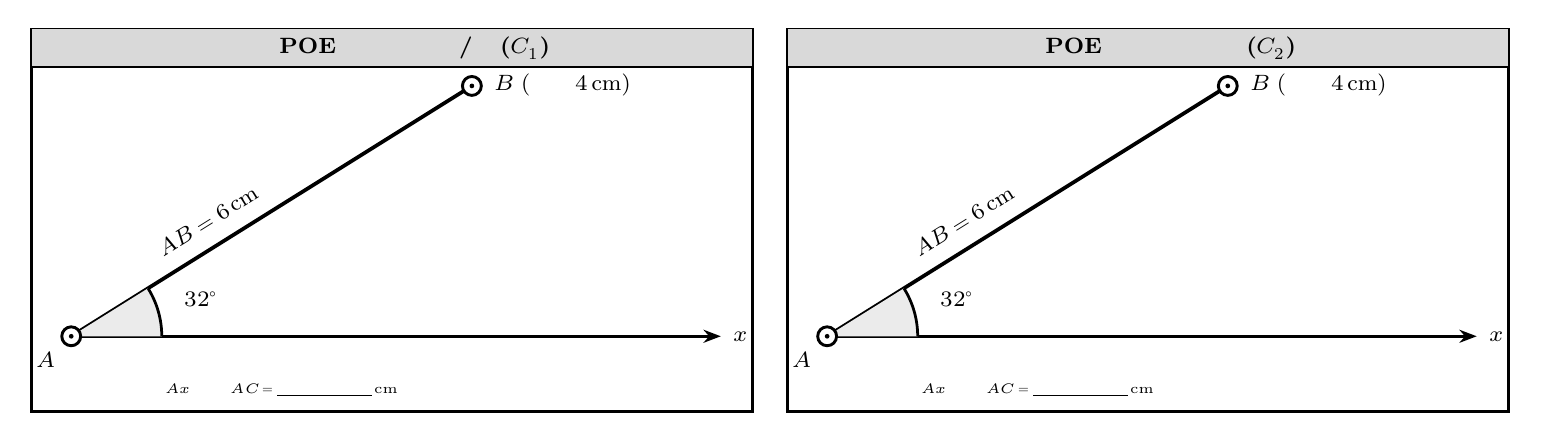
\begin{tikzpicture}[x=1cm, y=1cm, every node/.style={font=\scriptsize, text=black}]
  % ផ្ទាំងទី ១ (ខាងឆ្វេង) & ផ្ទាំងទី ២ (ខាងស្ដាំ)
  \foreach \xbase/\titletxt in {0.55/{ផ្ទាំង \en{POE} ទី ១ ៖ យោលកាត់កែង/ជិត ($C_1$)}, 10.15/{ផ្ទាំង \en{POE} ទី ២ ៖ យោលកាត់ឆ្ងាយ ($C_2$)}}{
    \begin{scope}[shift={(\xbase, 0)}]
      % ប្រអប់ផ្ទាំង (9.15 cm x 4.85 cm)
      \draw[black, line width=1.1pt] (-0.50, -0.95) rectangle (8.65, 3.90);
      \fill[headgray] (-0.50, 3.42) rectangle (8.65, 3.90);
      \draw[black, line width=0.9pt] (-0.50, 3.42) -- (8.65, 3.42);
      \node[font=\footnotesize] at (4.07, 3.66) {\textbf{\titletxt}};

      % ចំណុច A, B (AB = 6 cm, មុំ 32°) និងកន្លះបន្ទាត់ Ax
      \coordinate (A) at (0, 0);
      \coordinate (B) at (5.0883, 3.1795);
      \coordinate (Xend) at (8.25, 0);

      % កន្លះបន្ទាត់ Ax
      \draw[black, line width=1.15pt, -{Stealth[length=2.2mm]}] (A) -- (Xend);
      \node[right=1pt, font=\footnotesize] at (Xend) {$x$};

      % អង្កត់ AB = 6.0 cm នៅមុំ 32.0°
      \draw[black, line width=1.35pt] (A) -- (B);
      \node[above left=2pt, rotate=32, font=\footnotesize] at ($(A)!0.52!(B)$) {$AB = 6\unit{cm}$};

      % ធ្នូមុំ 32°
      \fill[panelgray] (A) -- (1.15, 0) arc (0:32:1.15) -- cycle;
      \draw[black, line width=1.0pt] (1.15, 0) arc (0:32:1.15);
      \node[font=\footnotesize] at (16:1.72) {$32^\circ$};

      % រន្ធម្ជុល o ត្រង់ A និង B
      \draw[black, line width=1.05pt, fill=white] (A) circle (0.12);
      \fill[black] (A) circle (0.03);
      \draw[black, line width=1.05pt, fill=white] (B) circle (0.12);
      \fill[black] (B) circle (0.03);

      \node[below left=2pt, font=\footnotesize] at (A) {$A$};
      \node[right=4.5pt, yshift=0.5pt, font=\footnotesize] at (B) {$B$ (ខ្ទាស់ $4\unit{cm}$)};

      % តំបន់យោលប៉ោលណែនាំខាងក្រោម Ax
      \node[font=\tiny, anchor=south west] at (0.15, -0.88) {គូសចំណុចប្រសព្វលើ $Ax$ រួចវាស់ $AC = \underline{\hspace{1.2cm}}\unit{cm}$};
    \end{scope}
  }
\end{tikzpicture}
\end{center}

\vspace{2pt}

% --- ផ្នែកទី ៣៖ តារាងកំណត់ត្រា POE (ទស្សន៍ទាយ - សង្កេត - ពន្យល់) ---
\begin{tcolorbox}[
  enhanced, sharp corners, colback=white, colframe=black,
  boxrule=1.05pt, top=4pt, bottom=4pt, left=6pt, right=6pt,
  title={\textbf{៣. តារាងកំណត់ត្រា \en{POE} (ទស្សន៍ទាយ — សង្កេត — ពន្យល់) សម្រាប់ពិសោធន៍ ១ \& ២}},
  colbacktitle=headgray, coltitle=black, fonttitle=\fontsize{9.2pt}{12pt}\selectfont
]
  \raggedright\fontsize{8.7pt}{12.8pt}\selectfont
  \textbf{\en{P} — ទស្សន៍ទាយ (មុនយោលបន្ទះ $4\unit{cm}$ ក្នុងពិសោធន៍ ២)៖} ដឹង $AB = 6\unit{cm}$, $BC = 4\unit{cm}$, $\ang{A} = 32^\circ$ តើបង្កើតបានប៉ុន្មានត្រីកោណ?\hspace{0.25cm}
  \mbox{\chkbox\ $0$} \hspace{0.25cm} \mbox{\chkbox\ $1$ ត្រីកោណតែមួយគត់} \hspace{0.25cm} \mbox{\chkbox\ $2$ ត្រីកោណខុសគ្នា}\\[4pt]
  \textbf{\en{O} — សង្កេត៖}
  \begin{itemize}[leftmargin=0.45cm, topsep=1pt, itemsep=2pt, parsep=0pt]
    \item \textbf{ពិសោធន៍ ១ (\en{SAS} ៖ ចាក់សោ $\ang{A} = 60^\circ$ រវាង $AB = 4\unit{cm}, AC = 6\unit{cm}$)៖} វាស់ $BC \approx \underline{\hspace{1.4cm}}\unit{cm}$ | ក្រដាសស្តើងបង្វិល-ត្រឡប់៖ \mbox{\chkbox\ ត្រួតស៊ីគ្នាបេះបិទ} \mbox{\chkbox\ ខុសគ្នា}
    \item \textbf{ពិសោធន៍ ២ (\en{SSA} ៖ យោល $BC = 4\unit{cm}$ ជុំវិញ $B$)៖} កាត់ $Ax$ ត្រង់ \mbox{\chkbox\ $1$ ចំណុច} \mbox{\chkbox\ $2$ ចំណុច ($C_1, C_2$)} | $AC_1 \approx \underline{\hspace{1.0cm}}\unit{cm}$, $AC_2 \approx \underline{\hspace{1.0cm}}\unit{cm}$ | $\tri{ABC_1}$ និង $\tri{ABC_2}$៖ \mbox{\chkbox\ ប៉ុនគ្នា} \mbox{\chkbox\ មិនប៉ុនគ្នា}
  \end{itemize}
  \vspace{2pt}
  \textbf{\en{E} — ពន្យល់៖} ហេតុអ្វីលក្ខខណ្ឌ \textbf{ជ-ម-ជ (\en{SAS})} ចាក់សោរាងត្រីកោណតែមួយគត់ ប៉ុន្តែ \textbf{ជ-ជ-ម (\en{SSA})} មិនអាចប្រើបាន?\\[5pt]
  \rule{\linewidth}{0.6pt}\\[8pt]
  \rule{\linewidth}{0.6pt}
\end{tcolorbox}

\clearpage

% ============================================================================
% ទំព័រទី ២៖ កាតស៊ើបអង្កេតសញ្ញាគន្លឹះ ៣ ជំហាន (ស-ខ្មៅ) — E4 Elaborate
% ============================================================================
\pagebanner{សម្ភារៈទី ២៖ កាតស៊ើបអង្កេតសញ្ញាគន្លឹះ ៣ ជំហាន (ស-ខ្មៅ)}{ទំព័រទី ២ / ៦ — សកម្មភាព \en{E4 Elaborate} (កាត់តាម \scissors)}

% --- ជួរខាងលើ៖ កាតទី ១ & កាតទី ២ ---
\noindent
\begin{tcolorbox}[
  enhanced, sharp corners, colback=white, colframe=white,
  borderline={0.95pt}{0pt}{black, dashed},
  width=9.25cm, equal height group=e4row1, nobeforeafter,
  top=4pt, bottom=4pt, left=5pt, right=5pt,
  title={\scissors\ \textbf{កាតទី ១៖ ករណីជ្រុងរួម \& ពុះមុំ (លំហាត់គំរូ \en{E4})}},
  colbacktitle=headgray, coltitle=black, fonttitle=\fontsize{8.8pt}{12pt}\selectfont
]
  \fontsize{8.3pt}{11.8pt}\selectfont
  គេឱ្យ $\ang{XOY}$ និងកន្លះបន្ទាត់ពុះ $OZ$ ។ លើ $OX, OY$ ដៅ $A, B$ ដែល $OA = OB$ និងដៅចំណុច $M \in OZ$ ។\\[2pt]
  ក. ប្រៀបធៀប $\tri{OMA}$ និង $\tri{OMB}$ ។\\
  ខ. ទាញបញ្ជាក់ថា $MA = MB$ និង $\ang{OAM} = \ang{OBM}$ ។
  \begin{center}
  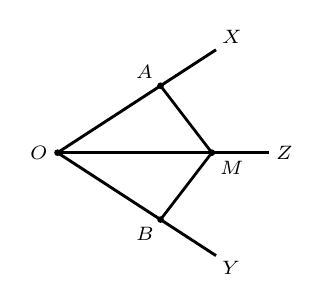
\begin{tikzpicture}[scale=0.80, every node/.style={font=\scriptsize, text=black}]
    \coordinate (O) at (0,0);
    \coordinate (X) at (33:3.0);
    \coordinate (Y) at (-33:3.0);
    \coordinate (Z) at (3.35,0);
    \coordinate (A) at (33:1.95);
    \coordinate (B) at (-33:1.95);
    \coordinate (M) at (2.45,0);
    \draw[black, line width=1.05pt] (O) -- (X);
    \draw[black, line width=1.05pt] (O) -- (Y);
    \draw[black, line width=1.15pt] (O) -- (Z);
    \draw[black, line width=1.0pt] (A) -- (M) -- (B);
    \fill[black] (O) circle (1.5pt) (A) circle (1.5pt) (B) circle (1.5pt) (M) circle (1.5pt);
    \node[left=2.5pt, inner sep=1pt] at (O) {$O$};
    \node[above left=1.5pt, inner sep=1pt] at (A) {$A$};
    \node[below left=1.5pt, inner sep=1pt] at (B) {$B$};
    \node[below right=2pt, inner sep=1pt] at (M) {$M$};
    \node[above right=1pt, inner sep=1pt] at (X) {$X$};
    \node[below right=1pt, inner sep=1pt] at (Y) {$Y$};
    \node[right=1.5pt, inner sep=1pt] at (Z) {$Z$};
  \end{tikzpicture}
  \end{center}
  \begin{tcolorbox}[enhanced, sharp corners, colback=panelgray, colframe=black, boxrule=0.7pt, top=3pt, bottom=3pt, left=4pt, right=4pt]
    \raggedright\fontsize{8.0pt}{12.0pt}\selectfont
    \textbf{ជំហាន ១ [ចង្អុលអូស + គូស \tickone\ និង \ticktwo]៖} ជ្រុងស្មើ ២ គូ៖\\
    (1) $\underline{\hspace{1.1cm}} = \underline{\hspace{1.1cm}}$ (\cnum{1}) \hspace{0.1cm} (2) $\underline{\hspace{1.1cm}} = \underline{\hspace{1.1cm}}$ (\cnum{3})\\[2pt]
    \textbf{ជំហាន ២ [ចង្អុលបត់ + ព័ទ្ធកំពូល \& ធ្នូ]៖}\\
    កំពូលរួម៖ $\underline{\hspace{0.7cm}}$ | មុំ៖ $\ang{\underline{\hspace{0.95cm}}} = \ang{\underline{\hspace{0.95cm}}}$ (\cnum{2})\\[2pt]
    \textbf{ជំហាន ៣ [ផ្ទៀង \en{S-A-S} \& សន្និដ្ឋាន]៖}\\
    មុំនៅចន្លោះជ្រុង? \mbox{\chkbox\ បាទ/ចាស (\en{SAS})} \mbox{\chkbox\ ទេ (អន្ទាក់ \en{SSA})}\\
    សន្និដ្ឋាន៖ $\tri{\underline{\hspace{0.95cm}}}\;\underline{\hspace{0.4cm}}\;\tri{\underline{\hspace{0.95cm}}}$ (\cnum{4}) $\Rightarrow MA=MB$ (\cnum{5})
  \end{tcolorbox}
\end{tcolorbox}%
\hfill
\begin{tcolorbox}[
  enhanced, sharp corners, colback=white, colframe=white,
  borderline={0.95pt}{0pt}{black, dashed},
  width=9.25cm, equal height group=e4row1, nobeforeafter,
  top=4pt, bottom=4pt, left=5pt, right=5pt,
  title={\scissors\ \textbf{កាតទី ២៖ ករណី \en{SAS} បង្វិល–ឆ្លុះ $140^\circ$ (បំបែកអគតិរូប)}},
  colbacktitle=headgray, coltitle=black, fonttitle=\fontsize{8.8pt}{12pt}\selectfont
]
  \fontsize{8.3pt}{11.8pt}\selectfont
  គេឱ្យ $\tri{ABC}$ និង $\tri{A'B'C'}$ ឆ្លុះនិងបង្វិល $140^\circ$ ដោយ $AB = A'B'$, $\ang{A} = \ang{A'}$, $AC = A'C'$ (ដូចរូប) ។ ចូរស៊ើបអង្កេតតាម ៣ ជំហាន និងផ្ទៀងលំដាប់កំពូល។
  \begin{center}
  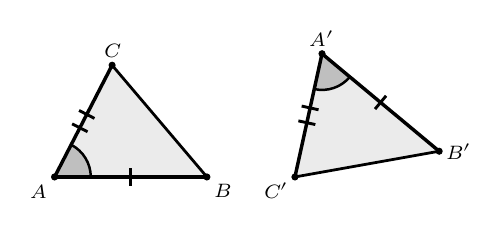
\begin{tikzpicture}[scale=0.86, every node/.style={font=\scriptsize, text=black}]
    % ត្រីកោណទី១
    \coordinate (A) at (0,0);
    \coordinate (B) at (2.25,0);
    \coordinate (C) at (0.85,1.65);
    \fill[panelgray] (A) -- (B) -- (C) -- cycle;
    \pic[draw=black, line width=0.9pt, fill=midgray, angle radius=4.6mm]{angle=B--A--C};
    \draw[black, line width=1.0pt] (B) -- (C);
    \draw[black, line width=1.25pt, tk1] (A) -- (B);
    \draw[black, line width=1.25pt, tk2] (A) -- (C);
    \fill[black] (A) circle (1.5pt) (B) circle (1.5pt) (C) circle (1.5pt);
    \node[below left=1.5pt, inner sep=1pt] at (A) {$A$};
    \node[below right=1.5pt, inner sep=1pt] at (B) {$B$};
    \node[above=1.5pt, inner sep=1pt] at (C) {$C$};
    % ត្រីកោណទី២ (ឆ្លុះ-បង្វិល 140 deg)
    \coordinate (Ap) at (3.95,1.82);
    \coordinate (Bp) at (5.68,0.38);
    \coordinate (Cp) at (3.55,0.00);
    \fill[panelgray] (Ap) -- (Bp) -- (Cp) -- cycle;
    \pic[draw=black, line width=0.9pt, fill=midgray, angle radius=4.6mm]{angle=Cp--Ap--Bp};
    \draw[black, line width=1.0pt] (Bp) -- (Cp);
    \draw[black, line width=1.25pt, tk1] (Ap) -- (Bp);
    \draw[black, line width=1.25pt, tk2] (Ap) -- (Cp);
    \fill[black] (Ap) circle (1.5pt) (Bp) circle (1.5pt) (Cp) circle (1.5pt);
    \node[above=1.5pt, inner sep=1pt] at (Ap) {$A'$};
    \node[right=1.5pt, inner sep=1pt] at (Bp) {$B'$};
    \node[below left=1pt, inner sep=1pt] at (Cp) {$C'$};
  \end{tikzpicture}
  \end{center}
  \vfill
  \begin{tcolorbox}[enhanced, sharp corners, colback=panelgray, colframe=black, boxrule=0.7pt, top=3pt, bottom=3pt, left=4pt, right=4pt]
    \raggedright\fontsize{8.0pt}{12.0pt}\selectfont
    \textbf{ជំហាន ១ [ចង្អុលអូសសញ្ញា \tickone\ និង \ticktwo]៖} ជ្រុងស្មើ ២ គូ៖\\
    (1) $\underline{\hspace{1.1cm}} = \underline{\hspace{1.1cm}}$ (\cnum{1}) \hspace{0.1cm} (2) $\underline{\hspace{1.1cm}} = \underline{\hspace{1.1cm}}$ (\cnum{1})\\[2pt]
    \textbf{ជំហាន ២ [ព័ទ្ធកំពូលជាប់ជ្រុងទាំងពីរ]៖}\\
    កំពូលរួម៖ $\underline{\hspace{0.6cm}}$ និង $\underline{\hspace{0.6cm}}$ | មុំ៖ $\ang{\underline{\hspace{0.8cm}}} = \ang{\underline{\hspace{0.8cm}}}$ (\cnum{1})\\[2pt]
    \textbf{ជំហាន ៣ [ផ្ទៀងលំដាប់កំពូល \& សន្និដ្ឋាន]៖}\\
    មុំនៅចន្លោះជ្រុង? \mbox{\chkbox\ បាទ/ចាស (\en{SAS})} \mbox{\chkbox\ ទេ (អន្ទាក់ \en{SSA})}\\
    សន្និដ្ឋាន៖ $\tri{\underline{\hspace{1.1cm}}}\;\underline{\hspace{0.5cm}}\;\tri{\underline{\hspace{1.1cm}}}$ (លេខ \cnum{4})
  \end{tcolorbox}
\end{tcolorbox}

\vspace{6pt}

% --- ជួរខាងក្រោម៖ កាតទី ៣ & កាតទី ៤ ---
\noindent
\begin{tcolorbox}[
  enhanced, sharp corners, colback=white, colframe=white,
  borderline={0.95pt}{0pt}{black, dashed},
  width=9.25cm, equal height group=e4row2, nobeforeafter,
  top=4pt, bottom=4pt, left=5pt, right=5pt,
  title={\scissors\ \textbf{កាតទី ៣៖ អន្ទាក់ ជ.ជ.ម (\en{SSA} មុំមិននៅចន្លោះ)}},
  colbacktitle=headgray, coltitle=black, fonttitle=\fontsize{8.8pt}{12pt}\selectfont
]
  \fontsize{8.3pt}{11.8pt}\selectfont
  គេសង់ $\tri{ABC_1}$ និង $\tri{ABC_2}$ ដោយដឹង $AB = 6\unit{cm}$, $BC_1 = BC_2 = 4\unit{cm}$ និង $\ang{A} = 32^\circ$ ។ តើ $\tri{ABC_1} \cg \tri{ABC_2}$ ដែរឬទេ?
  \begin{center}
  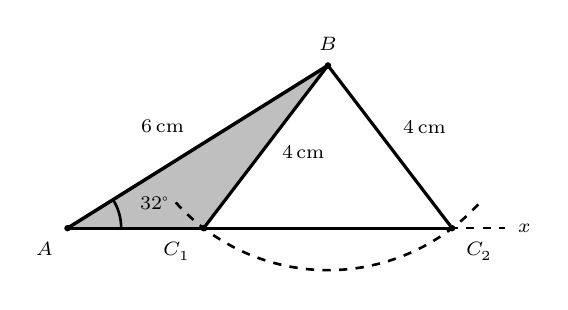
\begin{tikzpicture}[scale=0.65, every node/.style={font=\scriptsize, text=black}]
    \coordinate (A) at (0,0);
    \coordinate (B) at (5.0883, 3.1795);
    \coordinate (C1) at (2.6612, 0);
    \coordinate (C2) at (7.5154, 0);
    \coordinate (Xend) at (8.55, 0);
    \fill[midgray] (A) -- (B) -- (C1) -- cycle;
    \fill[white] (B) -- (C1) -- (C2) -- cycle;
    \draw[black, line width=0.95pt, dashed] (A) -- (Xend) node[right=1pt, font=\scriptsize] {$x$};
    \draw[black, line width=1.25pt] (A) -- (B) node[midway, above left=1pt, font=\scriptsize] {$6\unit{cm}$};
    \draw[black, line width=1.15pt] (B) -- (C1) node[midway, right=2pt, yshift=-2pt, font=\scriptsize] {$4\unit{cm}$};
    \draw[black, line width=1.15pt] (B) -- (C2) node[midway, above right=1pt, font=\scriptsize] {$4\unit{cm}$};
    \draw[black, line width=1.0pt] (A) -- (C2);
    \draw[black, line width=0.95pt, dashed] ($(B)+(-138:4)$) arc (-138:-42:4);
    \draw[black, line width=0.95pt] (1.05,0) arc (0:32:1.05);
    \node[font=\scriptsize] at (16:1.78) {$32^\circ$};
    \fill[black] (A) circle (1.8pt) node[below left=1.5pt] {$A$};
    \fill[black] (B) circle (1.8pt) node[above=2pt] {$B$};
    \fill[black] (C1) circle (1.8pt) node[below left=1.5pt] {$C_1$};
    \fill[black] (C2) circle (1.8pt) node[below right=1.5pt] {$C_2$};
  \end{tikzpicture}
  \end{center}
  \vfill
  \begin{tcolorbox}[enhanced, sharp corners, colback=panelgray, colframe=black, boxrule=0.7pt, top=3pt, bottom=3pt, left=4pt, right=4pt]
    \raggedright\fontsize{8.1pt}{12.0pt}\selectfont
    \textbf{ជំហាន ១ [ចង្អុលជ្រុងស្គាល់ ២]៖} $AB = 6\unit{cm}$ និង $BC = 4\unit{cm}$\\[2pt]
    \textbf{ជំហាន ២ [ព័ទ្ធកំពូលរួមនៃជ្រុងទាំង ២]៖}\\
    កំពូលរួមនៃ $AB, BC$ គឺ $\underline{\hspace{0.6cm}}$ | ប៉ុន្តែមុំស្គាល់គឺ $\ang{\underline{\hspace{0.6cm}}} = 32^\circ$\\[2pt]
    \textbf{ជំហាន ៣ [ផ្ទៀង \en{S-A-S} \& សន្និដ្ឋាន]៖}\\
    មុំនៅចន្លោះជ្រុង? \chkbox\ បាទ/ចាស (\en{SAS}) \chkbox\ ទេ (អន្ទាក់ \en{SSA})\\
    សន្និដ្ឋាន៖ $\tri{ABC_1}\;\underline{\hspace{0.5cm}}\;\tri{ABC_2}$ ព្រោះ $\underline{\hspace{2.6cm}}$
  \end{tcolorbox}
\end{tcolorbox}%
\hfill
\begin{tcolorbox}[
  enhanced, sharp corners, colback=white, colframe=white,
  borderline={0.95pt}{0pt}{black, dashed},
  width=9.25cm, equal height group=e4row2, nobeforeafter,
  top=4pt, bottom=4pt, left=5pt, right=5pt,
  title={\scissors\ \textbf{កាតទី ៤៖ ករណីមុំទល់កំពូល (រូបមេអំបៅ \en{E1/E5})}},
  colbacktitle=headgray, coltitle=black, fonttitle=\fontsize{8.8pt}{12pt}\selectfont
]
  \fontsize{8.3pt}{11.8pt}\selectfont
  គេមាន $\tri{AOB}$ ។ $A', B'$ ជាចំណុចឆ្លុះនៃ $A, B$ ធៀបនឹង $O$ ($OA = OA', OB = OB'$) ។ ចូររកមុំលាក់ត្រង់ $O$ ដើម្បីប្រៀបធៀប $\tri{OAB}$ និង $\tri{OA'B'}$ ។
  \begin{center}
  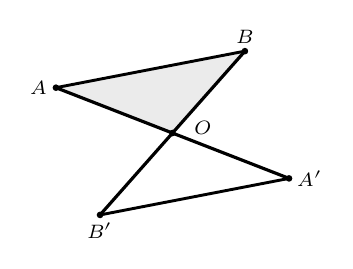
\begin{tikzpicture}[scale=0.80, every node/.style={font=\scriptsize, text=black}]
    \coordinate (O) at (0,0);
    \coordinate (A) at (-1.85, 0.72);
    \coordinate (B) at (1.15, 1.30);
    \coordinate (Ap) at (1.85, -0.72);
    \coordinate (Bp) at (-1.15, -1.30);
    \fill[panelgray] (O) -- (A) -- (B) -- cycle;
    \fill[white] (O) -- (Ap) -- (Bp) -- cycle;
    \draw[black, line width=1.15pt] (A) -- (Ap);
    \draw[black, line width=1.15pt] (B) -- (Bp);
    \draw[black, line width=1.05pt] (A) -- (B) (Ap) -- (Bp);
    \fill[black] (O) circle (1.5pt) (A) circle (1.5pt) (B) circle (1.5pt) (Ap) circle (1.5pt) (Bp) circle (1.5pt);
    \node[left=2pt, inner sep=1pt] at (A) {$A$};
    \node[above=1.5pt, inner sep=1pt] at (B) {$B$};
    \node[right=2pt, inner sep=1pt] at (Ap) {$A'$};
    \node[below=1.5pt, inner sep=1pt] at (Bp) {$B'$};
    \node[right=4.5pt, yshift=2pt, font=\scriptsize] at (O) {$O$};
  \end{tikzpicture}
  \end{center}
  \vfill
  \begin{tcolorbox}[enhanced, sharp corners, colback=panelgray, colframe=black, boxrule=0.7pt, top=3pt, bottom=3pt, left=4pt, right=4pt]
    \raggedright\fontsize{8.0pt}{12.0pt}\selectfont
    \textbf{ជំហាន ១ [គូស \tickone\ និង \ticktwo\ លើរូប (ហាមគូស $AB=A'B'$)]៖}\\
    (1) $\underline{\hspace{1.1cm}} = \underline{\hspace{1.1cm}}$ (\cnum{1}) \hspace{0.1cm} (2) $\underline{\hspace{1.1cm}} = \underline{\hspace{1.1cm}}$ (\cnum{1})\\[2pt]
    \textbf{ជំហាន ២ [ព័ទ្ធកំពូល $O$ \& គូសធ្នូមុំលាក់]៖}\\
    កំពូលរួម៖ $\underline{\hspace{0.6cm}}$ | មុំ៖ $\ang{\underline{\hspace{0.95cm}}} = \ang{\underline{\hspace{0.95cm}}}$ (\cnum{2} ទល់កំពូល)\\[2pt]
    \textbf{ជំហាន ៣ [ផ្ទៀង \en{S-A-S} \& សន្និដ្ឋាន]៖}\\
    មុំនៅចន្លោះជ្រុង? \mbox{\chkbox\ បាទ/ចាស (\en{SAS})} \mbox{\chkbox\ ទេ (អន្ទាក់ \en{SSA})}\\
    សន្និដ្ឋាន៖ $\tri{\underline{\hspace{1.1cm}}}\;\underline{\hspace{0.5cm}}\;\tri{\underline{\hspace{1.1cm}}}$ (លេខ \cnum{4})
  \end{tcolorbox}
\end{tcolorbox}

\clearpage

% ============================================================================
% ទំព័រទី ៣៖ សន្លឹកកិច្ចការប្រលង Relay ក្រុម ៣ តួនាទី — E5 Evaluate
% ============================================================================
\pagebanner{សម្ភារៈទី ៣៖ សន្លឹកកិច្ចការប្រលង \en{Relay} ក្រុម ៣ តួនាទី}{ទំព័រទី ៣ / ៦ — សកម្មភាព \en{E5 Evaluate}}

% --- ព័ត៌មានក្រុម & ធនាគារហេតុផល ---
\begin{tcolorbox}[
  enhanced, sharp corners, colback=panelgray, colframe=black,
  boxrule=0.95pt, top=3.5pt, bottom=3.5pt, left=6pt, right=6pt, after skip=5pt
]
  \fontsize{8.5pt}{12.5pt}\selectfont
  \textbf{ក្រុមវិស្វករ៖} $\underline{\hspace{2.6cm}}$ | \textbf{អ្នកទី ១ (\en{Visual Marker})៖} $\underline{\hspace{2.0cm}}$ | \textbf{អ្នកទី ២ (\en{Warrant})៖} $\underline{\hspace{2.0cm}}$ | \textbf{អ្នកទី ៣ (\en{Order})៖} $\underline{\hspace{2.0cm}}$\\[2pt]
  \textbf{ធនាគារអំណះអំណាង៖} \cnum{1} បម្រាប់/ឆ្លុះ \hspace{0.2cm} \cnum{2} មុំទល់កំពូល/ពុះមុំ \hspace{0.2cm} \cnum{3} ជ្រុងរួម \hspace{0.2cm} \cnum{4} លក្ខខណ្ឌ ជ.ម.ជ (\en{SAS}) \hspace{0.2cm} \cnum{5} ធាតុត្រូវគ្នា \hspace{0.25cm}|\hspace{0.25cm} \textbf{សម្គាល់៖} $=$ ប្រវែង/រង្វាស់, $\cg$ ត្រីកោណប៉ុនគ្នា
\end{tcolorbox}

% --- ភារកិច្ច A (Task A) ---
\begin{tcolorbox}[
  enhanced, sharp corners, colback=white, colframe=black,
  boxrule=1.05pt, top=3pt, bottom=3pt, left=5pt, right=5pt, after skip=5pt,
  title={\textbf{ភារកិច្ច \en{A} (\en{Task A}) — លំហាត់ប្រតិបត្តិ \en{E5}៖} គេមាន $\tri{AOB}$ ។ $A', B'$ ជាចំណុចឆ្លុះនៃ $A, B$ ធៀប $O$ ។ បង្ហាញ $\tri{OAB}\cg\tri{OA'B'}$ រួចទាញ $AB=A'B'$ ។},
  colbacktitle=headgray, coltitle=black, fonttitle=\fontsize{8.5pt}{11.5pt}\selectfont
]
  \renewcommand{\arraystretch}{1.10}
  \begin{tabular}{|L{5.4cm}|L{6.5cm}|L{5.2cm}|}
    \hline
    \cellcolor{panelgray}\centering\arraybackslash\textbf{តួនាទី ១ (\en{Visual Marker})}\newline {\fontsize{7.6pt}{9.5pt}\selectfont ៣០ វិនាទី — ពន្យល់មាត់មុនគូសលើរូប} &
    \cellcolor{panelgray}\centering\arraybackslash\textbf{តួនាទី ២ (\en{Warrant Connector} \cnum{1}--\cnum{5})}\newline {\fontsize{7.6pt}{9.5pt}\selectfont \textbf{\en{Pause-Ask!}} — សួរផ្ទៀងមុនសរសេរ} &
    \cellcolor{panelgray}\centering\arraybackslash\textbf{តួនាទី ៣ (\en{Order Checker})}\newline {\fontsize{7.6pt}{9.5pt}\selectfont \textbf{\en{Pause-Review!}} — ផ្ទៀងលំដាប់ \& វិបាក} \\ \hline
    {\centering
    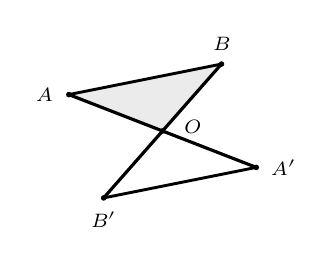
\begin{tikzpicture}[scale=0.68, every node/.style={font=\scriptsize, text=black}]
      \coordinate (O) at (0,0);
      \coordinate (A) at (-1.75, 0.68);
      \coordinate (B) at (1.10, 1.25);
      \coordinate (Ap) at (1.75, -0.68);
      \coordinate (Bp) at (-1.10, -1.25);
      \fill[panelgray] (O) -- (A) -- (B) -- cycle;
      \fill[white] (O) -- (Ap) -- (Bp) -- cycle;
      \draw[black, line width=1.15pt] (A) -- (Ap);
      \draw[black, line width=1.15pt] (B) -- (Bp);
      \draw[black, line width=1.05pt] (A) -- (B) (Ap) -- (Bp);
      \fill[black] (O) circle (1.5pt) (A) circle (1.5pt) (B) circle (1.5pt) (Ap) circle (1.5pt) (Bp) circle (1.5pt);
      \node[left=2pt] at (A) {$A$};
      \node[above=1.5pt] at (B) {$B$};
      \node[right=2pt] at (Ap) {$A'$};
      \node[below=1.5pt] at (Bp) {$B'$};
      \node[right=4.5pt, yshift=1.5pt] at (O) {$O$};
    \end{tikzpicture}\par}
    \vspace{2pt}\fontsize{7.8pt}{11.2pt}\selectfont
    \chkbox\ គូស \tickone\ លើ $OA = OA'$\newline
    \chkbox\ គូស \ticktwo\ លើ $OB = OB'$\newline
    \chkbox\ ព័ទ្ធកំពូល $O$ \& គូសធ្នូ \cnum{2} មុំទល់កំពូល\newline
    \chkbox\ \textbf{ហាមគូស} $AB = A'B'$ (មិនទាន់ដឹង!)
    &
    \fontsize{8.0pt}{12.5pt}\selectfont
    \textbf{\en{Pause-Ask!}} សួរដៃគូមុនសរសេរ៖\newline
    «ហេតុអ្វី $\ang{AOB}=\ang{A'OB'}$? តើ $O$ នៅចន្លោះជ្រុងឬ?»\par\vspace{3pt}
    ក្នុង $\tri{\underline{\hspace{0.95cm}}}$ និង $\tri{\underline{\hspace{0.95cm}}}$ មាន៖\par\vspace{3pt}
    \en{1)} $\underline{\hspace{1.45cm}} = \underline{\hspace{1.45cm}}$ (\cnum{1} $\underline{\hspace{1.4cm}}$)\par\vspace{3pt}
    \en{2)} $\ang{\underline{\hspace{1.15cm}}} = \ang{\underline{\hspace{1.15cm}}}$ (\cnum{2} $\underline{\hspace{1.4cm}}$)\par\vspace{3pt}
    \en{3)} $\underline{\hspace{1.45cm}} = \underline{\hspace{1.45cm}}$ (\cnum{1} $\underline{\hspace{1.4cm}}$)\par\vspace{4pt}
    ដូចនេះ $\tri{\underline{\hspace{1.05cm}}} \cg \tri{\underline{\hspace{1.05cm}}}$ (\cnum{4} $\underline{\hspace{1.15cm}}$)
    &
    \fontsize{8.0pt}{12.5pt}\selectfont
    \textbf{\en{Pause-Review!}} ផ្ទៀងមុនបញ្ចប់៖\newline
    \chkbox\ លំដាប់កំពូល៖\newline
    \hspace*{0.2cm}$O \to \underline{\hspace{0.45cm}} \to \underline{\hspace{0.45cm}}$ ទល់ $O \to \underline{\hspace{0.45cm}} \to \underline{\hspace{0.45cm}}$\newline
    \chkbox\ ប្រើ $=$ លើប្រវែង/មុំ និង $\cg$ លើត្រីកោណ\par\vspace{4pt}
    \textbf{ទាញវិបាក (\cnum{5} ធាតុត្រូវគ្នា)៖}\par\vspace{2pt}
    \en{1)} $AB = \underline{\hspace{1.7cm}}$\par\vspace{3pt}
    \en{2)} $\ang{OAB} = \ang{\underline{\hspace{1.3cm}}}$\par\vspace{3pt}
    \en{3)} $\ang{OBA} = \ang{\underline{\hspace{1.3cm}}}$
    \\[2pt] \hline
  \end{tabular}
\end{tcolorbox}

% --- ភារកិច្ច B (Task B) ---
\begin{tcolorbox}[
  enhanced, sharp corners, colback=white, colframe=black,
  boxrule=1.05pt, top=3pt, bottom=3pt, left=5pt, right=5pt,
  title={\textbf{ភារកិច្ច \en{B} (\en{Task B}) — បិទបញ្ចប់បេសកកម្ម \en{E1} (វាស់ទទឹងស្រះទឹក)៖} វិស្វករដៅ $O$ វាស់ $OA'=OA$, $OB'=OB$ និង $A'B'=18\unit{m}$ ។ ពិនិត្យ $\tri{OA'B'}$ និង $\tri{OAB}$ ដើម្បីរកទទឹងស្រះ $AB$ ។},
  colbacktitle=headgray, coltitle=black, fonttitle=\fontsize{8.5pt}{11.5pt}\selectfont
]
  \renewcommand{\arraystretch}{1.10}
  \begin{tabular}{|L{5.4cm}|L{6.5cm}|L{5.2cm}|}
    \hline
    \cellcolor{panelgray}\centering\arraybackslash\textbf{តួនាទី ១ (\en{Visual Marker})}\newline {\fontsize{7.6pt}{9.5pt}\selectfont ៣០ វិនាទី — ពន្យល់មាត់មុនគូសលើរូប} &
    \cellcolor{panelgray}\centering\arraybackslash\textbf{តួនាទី ២ (\en{Warrant Connector} \cnum{1}--\cnum{5})}\newline {\fontsize{7.6pt}{9.5pt}\selectfont \textbf{\en{Pause-Ask!}} — សួរផ្ទៀងមុនសរសេរ} &
    \cellcolor{panelgray}\centering\arraybackslash\textbf{តួនាទី ៣ (\en{Order Checker})}\newline {\fontsize{7.6pt}{9.5pt}\selectfont \textbf{\en{Pause-Review!}} — ផ្ទៀងលំដាប់ \& បិទ \en{E1}} \\ \hline
    {\centering
    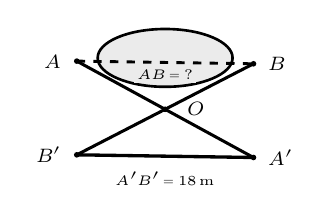
\begin{tikzpicture}[scale=0.68, every node/.style={font=\scriptsize, text=black}]
      \coordinate (O) at (0,0);
      \coordinate (A) at (-1.65, 0.90);
      \coordinate (B) at (1.65, 0.85);
      \coordinate (Ap) at (1.65, -0.90);
      \coordinate (Bp) at (-1.65, -0.85);
      \fill[panelgray, draw=black, line width=0.95pt] (0, 0.96) ellipse (1.26cm and 0.54cm);
      \node[font=\tiny] at (0, 1.24) {ស្រះទឹក};
      \draw[black, line width=1.1pt] (A) -- (Ap);
      \draw[black, line width=1.1pt] (B) -- (Bp);
      \draw[black, line width=1.05pt, dashed] (A) -- (B);
      \draw[black, line width=1.2pt] (Bp) -- (Ap);
      \fill[black] (O) circle (1.5pt) (A) circle (1.5pt) (B) circle (1.5pt) (Ap) circle (1.5pt) (Bp) circle (1.5pt);
      \node[right=4.5pt, font=\scriptsize] at (O) {$O$};
      \node[left=2pt] at (A) {$A$};
      \node[right=2pt] at (B) {$B$};
      \node[right=2pt] at (Ap) {$A'$};
      \node[left=2pt] at (Bp) {$B'$};
      \node[fill=panelgray, inner sep=1pt, font=\tiny] at (0, 0.64) {$AB = ?$};
      \node[below=2pt, font=\tiny] at ($(Bp)!0.5!(Ap)$) {$A'B' = 18\unit{m}$};
    \end{tikzpicture}\par}
    \vspace{2pt}\fontsize{7.8pt}{11.2pt}\selectfont
    \chkbox\ គូស \tickone\ លើ $OA' = OA$\newline
    \chkbox\ គូស \ticktwo\ លើ $OB' = OB$\newline
    \chkbox\ ព័ទ្ធ $O$ \& គូសធ្នូ $\ang{A'OB'}=\ang{AOB}$ (\cnum{2})\newline
    \chkbox\ \textbf{ហាមគូស} $AB=18\unit{m}$ លើរូបមុនស្រាយ!
    &
    \fontsize{8.0pt}{12.5pt}\selectfont
    \textbf{\en{Pause-Ask!}} សួរដៃគូមុនសរសេរ៖\newline
    «តើជ្រុង $OA', OB'$ អមជុំវិញមុំ $\ang{A'OB'}$ មែនឬ?»\par\vspace{3pt}
    ពិនិត្យ $\tri{OA'B'}$ និង $\tri{OAB}$ មាន៖\par\vspace{3pt}
    \en{1)} $OA' = \underline{\hspace{1.25cm}}$ (\cnum{1} បម្រាប់វាស់)\par\vspace{3pt}
    \en{2)} $\ang{A'OB'} = \ang{\underline{\hspace{1.0cm}}}$ (\cnum{2} $\underline{\hspace{1.4cm}}$)\par\vspace{3pt}
    \en{3)} $OB' = \underline{\hspace{1.25cm}}$ (\cnum{1} បម្រាប់វាស់)\par\vspace{4pt}
    $\Rightarrow \tri{\underline{\hspace{1.05cm}}} \cg \tri{\underline{\hspace{1.05cm}}}$ (\cnum{4} $\underline{\hspace{1.15cm}}$)
    &
    \fontsize{8.0pt}{12.5pt}\selectfont
    \textbf{\en{Pause-Review!}} ផ្ទៀងលំដាប់បញ្ច្រាស៖\newline
    \chkbox\ $O \to A' \to B'$ ទល់ $O \to \underline{\hspace{0.45cm}} \to \underline{\hspace{0.45cm}}$\newline
    \chkbox\ ប្រើ $=$ និង $\cg$ បានត្រឹមត្រូវ\par\vspace{4pt}
    \textbf{សន្និដ្ឋានទទឹងស្រះ (\cnum{5})៖}\par\vspace{2pt}
    $AB = A'B' = \underline{\hspace{1.3cm}}\unit{m}$\par\vspace{4pt}
    \textbf{ទំហំត្រីកោណពិត៖}\par\vspace{2pt}
    $\ang{OAB} = \ang{\underline{\hspace{1.0cm}}}$, $\ang{OBA} = \ang{\underline{\hspace{1.0cm}}}$
    \\[2pt] \hline
  \end{tabular}
\end{tcolorbox}

\clearpage

% ============================================================================
% ទំព័រទី ៤៖ ផ្ទាំងយោងប្រចាំថ្នាក់រៀន — ធនាគារអំណះអំណាង ①–⑤ & វិធីផ្ទៀងមុំចន្លោះ
% ============================================================================
\begin{tcolorbox}[
  enhanced, sharp corners, colback=white, colframe=black,
  boxrule=1.5pt, borderline={0.6pt}{2.2pt}{black},
  top=5pt, bottom=5pt, left=7pt, right=7pt
]
  \begin{center}
    {\muol\fontsize{12pt}{17pt}\selectfont ធនាគារអំណះអំណាង \cnum{1}--\cnum{5} និងវិធីផ្ទៀងមុំចន្លោះ}\\[1pt]
    {\fontsize{9pt}{13pt}\selectfont ផ្ទាំងយោងប្រចាំថ្នាក់រៀន (ស-ខ្មៅ) — មេរៀនទី១២ (១.២.២) ករណីត្រីកោណប៉ុនគ្នា \textbf{ជ.ម.ជ (\en{SAS})}}\\[3pt]
    \khmflourish
  \end{center}
  \vspace{1pt}
  {\fontsize{8.6pt}{12.5pt}\selectfont
  \textbf{ទ្រឹស្ដីបទ (ជ.ម.ជ)៖} ត្រីកោណពីរប៉ុនគ្នា កាលណាវាមានមុំមួយប៉ុនគ្នា អមដោយជ្រុងពីរប៉ុនរៀងគ្នា ។ \hspace{0.3cm} \textbf{គោលការណ៍កំពូលរួម៖} កំពូលមុំត្រូវជាប់ចន្លោះជ្រុងទាំងពីរជានិច្ច (\en{S--A--S}) ។}

  \vspace{4pt}

  % --- តារាងធនាគារអំណះអំណាង ①–⑤ ជាមួយរូប TikZ ស-ខ្មៅ ---
  \fontsize{8.3pt}{11.8pt}\selectfont
  \renewcommand{\arraystretch}{1.10}
  \begin{tabular}{|C{0.9cm}|L{3.8cm}|L{6.2cm}|C{5.6cm}|}
    \hline
    \cellcolor{headgray}\textbf{លេខ} &
    \cellcolor{headgray}\centering\arraybackslash\textbf{ឈ្មោះអំណះអំណាង} &
    \cellcolor{headgray}\centering\arraybackslash\textbf{និមិត្តសញ្ញា និងរបៀបសរសេរ} &
    \cellcolor{headgray}\centering\arraybackslash\textbf{រូបសម្គាល់ ស-ខ្មៅ} \\ \hline

    \cnum{1} &
    \textbf{បម្រាប់ / សម្មតិកម្ម}\newline (\en{Given / Reflection}) &
    ប្រវែងជ្រុង ឬរង្វាស់មុំដែលប្រធានឱ្យស្រាប់ ឬឆ្លុះធៀបចំណុច (ឧ. $AB=A'B'$, $OA=OA'$)។ គូស \tickone\ ឬ \ticktwo\ ។ &
    \raisebox{-0.4\height}{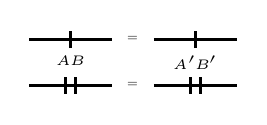
\begin{tikzpicture}[scale=0.66, every node/.style={font=\scriptsize, text=black}]
      \draw[black, line width=1.15pt, tk1] (0,0.48) -- (1.6,0.48);
      \draw[black, line width=1.15pt, tk1] (2.4,0.48) -- (4.0,0.48);
      \node[below=1.5pt, font=\tiny] at (0.8,0.44) {$AB$};
      \node[below=1.5pt, font=\tiny] at (3.2,0.44) {$A'B'$};
      \node[font=\tiny] at (2.0,0.48) {$=$};
      \draw[black, line width=1.15pt, tk2] (0,-0.40) -- (1.6,-0.40);
      \draw[black, line width=1.15pt, tk2] (2.4,-0.40) -- (4.0,-0.40);
      \node[font=\tiny] at (2.0,-0.40) {$=$};
    \end{tikzpicture}} \\ \hline

    \cnum{2} &
    \textbf{មុំទល់កំពូល / ពុះមុំ}\newline (\en{Vertical / Bisector}) &
    \textbullet\ មុំទល់កំពូល៖ $\ang{AOB}=\ang{A'OB'}$\newline
    \textbullet\ កន្លះបន្ទាត់ពុះមុំ៖ $\ang{XOZ}=\ang{ZOY}$ (ព័ទ្ធកំពូល \& គូសធ្នូមុំស្មើ)។ &
    \raisebox{-0.4\height}{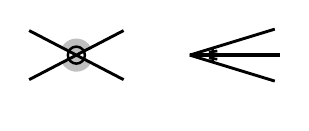
\begin{tikzpicture}[scale=0.60, every node/.style={font=\scriptsize, text=black}]
      % មុំទល់កំពូល
      \begin{scope}[shift={(-1.7,0)}]
        \fill[midgray] (0,0) -- (150:0.35) arc (150:25:0.35) -- cycle;
        \fill[midgray] (0,0) -- (-30:0.35) arc (-30:-155:0.35) -- cycle;
        \draw[black, line width=1.05pt] (-1.0,0.52) -- (1.0,-0.52) (-1.0,-0.52) -- (1.0,0.52);
        \draw[black, line width=0.9pt] (0,0) circle (0.18);
        \node[below=6pt, font=\tiny] at (0,-0.25) {ទល់កំពូល};
      \end{scope}
      % ពុះមុំ
      \begin{scope}[shift={(1.5,0)}]
        \draw[black, line width=1.05pt] (-0.8,0) -- (1.0,0.55) (-0.8,0) -- (1.0,-0.55);
        \draw[black, line width=1.2pt] (-0.8,0) -- (1.1,0);
        \draw[black, line width=0.9pt] ($(-0.8,0)+(17:0.50)$) arc (17:-17:0.50);
        \draw[black, line width=0.95pt] ($(-0.8,0)+(8.5:0.41)$) -- ($(-0.8,0)+(8.5:0.59)$);
        \draw[black, line width=0.95pt] ($(-0.8,0)+(-8.5:0.41)$) -- ($(-0.8,0)+(-8.5:0.59)$);
        \node[below=6pt, font=\tiny] at (0.1,-0.25) {កន្លះបន្ទាត់ពុះមុំ};
      \end{scope}
    \end{tikzpicture}} \\ \hline

    \cnum{3} &
    \textbf{ជ្រុងរួម / កំពូលរួម}\newline (\en{Reflexive Side}) &
    ជ្រុងជាប់គ្នាក្នុងត្រីកោណទាំងពីរ៖ $OM = OM$ ឬ $AD = AD$ ។ ចង្អុលអូស + គូស \ticktwo\ លើជ្រុងកណ្ដាល! &
    \raisebox{-0.4\height}{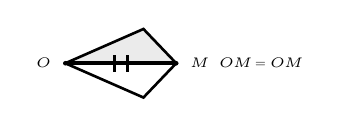
\begin{tikzpicture}[scale=0.64, every node/.style={font=\scriptsize, text=black}]
      \coordinate (O) at (0,0);
      \coordinate (M) at (2.2,0);
      \coordinate (A) at (1.55,0.68);
      \coordinate (B) at (1.55,-0.68);
      \fill[panelgray] (O) -- (M) -- (A) -- cycle;
      \draw[black, line width=0.95pt] (O) -- (A) -- (M) -- (B) -- (O);
      \draw[black, line width=1.35pt, tk2] (O) -- (M);
      \fill[black] (O) circle (1.3pt) (M) circle (1.3pt);
      \node[left=1.5pt, font=\tiny] at (O) {$O$};
      \node[right=1.5pt, font=\tiny] at (M) {$M$};
      \node[right=12pt, font=\tiny] at (M) {$OM=OM$};
    \end{tikzpicture}} \\ \hline

    \cnum{4} &
    \textbf{លក្ខខណ្ឌ ជ.ម.ជ (\en{SAS})}\newline (\en{Included Angle}) &
    ជ្រុង--មុំចន្លោះ--ជ្រុង ទាញ $\tri{ABC} \cg \tri{A'B'C'}$ ។ ផ្ទៀងតាមលំដាប់កំពូល ទោះរូបបង្វិល–ឆ្លុះ $140^\circ$! &
    \raisebox{-0.4\height}{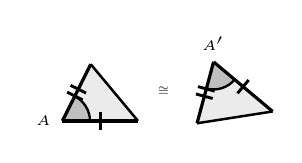
\begin{tikzpicture}[scale=0.60, every node/.style={font=\scriptsize, text=black}]
      \coordinate (A) at (0,0); \coordinate (B) at (1.6,0); \coordinate (C) at (0.6,1.2);
      \fill[panelgray] (A)--(B)--(C)--cycle;
      \pic[draw=black, line width=0.85pt, fill=midgray, angle radius=3.5mm]{angle=B--A--C};
      \draw[black, line width=0.9pt] (B)--(C);
      \draw[black, line width=1.15pt, tk1] (A)--(B);
      \draw[black, line width=1.15pt, tk2] (A)--(C);
      \node[left=0.5pt, font=\tiny] at (A) {$A$};
      \coordinate (Ap) at (3.2,1.25); \coordinate (Bp) at (4.45,0.20); \coordinate (Cp) at (2.85,-0.05);
      \fill[panelgray] (Ap)--(Bp)--(Cp)--cycle;
      \pic[draw=black, line width=0.85pt, fill=midgray, angle radius=3.5mm]{angle=Cp--Ap--Bp};
      \draw[black, line width=0.9pt] (Bp)--(Cp);
      \draw[black, line width=1.15pt, tk1] (Ap)--(Bp);
      \draw[black, line width=1.15pt, tk2] (Ap)--(Cp);
      \node[above=0.5pt, font=\tiny] at (Ap) {$A'$};
      \node[font=\tiny] at (2.15, 0.65) {$\cg$};
    \end{tikzpicture}} \\ \hline

    \cnum{5} &
    \textbf{ធាតុត្រូវគ្នា}\newline (\en{Consequence}) &
    ពេល $\tri{ABC}\cg\tri{A'B'C'}$ ទាញបានធាតុ ៣ នៅសល់៖ $BC=B'C'$, $\ang{B}=\ang{B'}$, $\ang{C}=\ang{C'}$ ។ &
    \raisebox{-0.4\height}{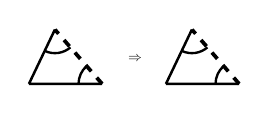
\begin{tikzpicture}[scale=0.60, every node/.style={font=\scriptsize, text=black}]
      \coordinate (A) at (0,0); \coordinate (B) at (1.55,0); \coordinate (C) at (0.55,1.15);
      \draw[black, line width=0.9pt] (A)--(B) (A)--(C);
      \draw[black, line width=1.35pt, dashed] (B)--(C);
      \pic[draw=black, line width=0.85pt, angle radius=3.0mm]{angle=C--B--A};
      \pic[draw=black, line width=0.85pt, angle radius=3.0mm]{angle=A--C--B};
      \node[font=\tiny] at (2.25, 0.55) {$\Rightarrow$};
      \coordinate (D) at (2.9,0); \coordinate (E) at (4.45,0); \coordinate (F) at (3.45,1.15);
      \draw[black, line width=0.9pt] (D)--(E) (D)--(F);
      \draw[black, line width=1.35pt, dashed] (E)--(F);
      \pic[draw=black, line width=0.85pt, angle radius=3.0mm]{angle=F--E--D};
      \pic[draw=black, line width=0.85pt, angle radius=3.0mm]{angle=D--F--E};
    \end{tikzpicture}} \\ \hline
  \end{tabular}

  \vspace{5pt}

  % --- វិធីផ្ទៀងមុំចន្លោះ ៣ ជំហាន & សញ្ញា = vs \cong ---
  \begin{tcolorbox}[
    enhanced, sharp corners, colback=panelgray, colframe=black,
    boxrule=0.95pt, top=4pt, bottom=4pt, left=6pt, right=6pt, after skip=5pt
  ]
    \fontsize{8.6pt}{12.5pt}\selectfont
    \textbf{វិធីផ្ទៀងមុំចន្លោះ ៣ ជំហាន (គោលការណ៍កំពូលរួម)៖}\\[2pt]
    \textbf{១.} រកអក្សរកំពូលរួមនៃជ្រុងទាំង ២ ក្នុងត្រីកោណនីមួយៗ (ឧ. $AB$ និង $AC$ មានកំពូលរួម \textbf{$A$})។ \hspace{0.2cm}
    \textbf{២.} ចង្អុលអូសតាម \en{S--A--S}៖ មុំត្រូវតែជាកំពូលរួម $\ang{A}$ នោះ!\\
    \textbf{៣.} ផ្ទៀងលំដាប់កំពូលឆ្លងត្រីកោណ ($A\to B\to C$ ទល់ $A'\to B'\to C'$) និងបែងចែកសញ្ញា៖ \textbf{$=$} សម្រាប់ប្រវែង/រង្វាស់មុំ \hspace{0.2cm} និង \hspace{0.2cm} \textbf{$\cg$} សម្រាប់ត្រីកោណប៉ុនគ្នា!
  \end{tcolorbox}

  % --- ប្រអប់ព្រមានផ្ទឹមគ្នា៖ ជ-ម-ជ (SAS) vs ជ-ជ-ម (SSA មិនស្មើគ្នា) ---
  \noindent
  \begin{minipage}[t]{8.8cm}
    \begin{tcolorbox}[
      enhanced, sharp corners, colback=white, colframe=black,
      boxrule=1.2pt, equal height group=posterwarn,
      top=3pt, bottom=4pt, left=5pt, right=5pt,
      title={\ding{51}\ \textbf{ត្រូវ៖ ករណី ជ-ម-ជ (\en{SAS}) — ប៉ុនគ្នា!}},
      colbacktitle=headgray, coltitle=black, fonttitle=\fontsize{8.8pt}{12pt}\selectfont
    ]
      \centering
      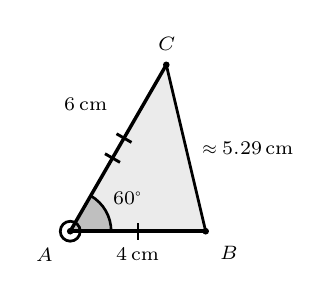
\begin{tikzpicture}[scale=0.80, every node/.style={font=\scriptsize, text=black}]
        \coordinate (A) at (0,0);
        \coordinate (B) at (2.15,0);
        \coordinate (C) at (60:3.05);
        \fill[panelgray] (A) -- (B) -- (C) -- cycle;
        \fill[midgray] (A) -- (0.65,0) arc (0:60:0.65) -- cycle;
        \draw[black, line width=0.95pt] (0.65,0) arc (0:60:0.65);
        \draw[black, line width=1.25pt, tk1] (A) -- (B) node[midway, below=2pt] {$4\unit{cm}$};
        \draw[black, line width=1.25pt, tk2] (A) -- (C) node[pos=0.60, above left=3.5pt] {$6\unit{cm}$};
        \draw[black, line width=1.0pt] (B) -- (C) node[midway, right=2pt] {$\approx 5.29\unit{cm}$};
        \draw[black, line width=1.0pt] (A) circle (4.5pt);
        \fill[black] (A) circle (1.5pt) (B) circle (1.5pt) (C) circle (1.5pt);
        \node[below left=2.5pt] at (A) {$A$};
        \node[below right=2pt] at (B) {$B$};
        \node[above=1.5pt] at (C) {$C$};
        \node[font=\scriptsize] at (30:1.05) {$60^\circ$};
      \end{tikzpicture}
      \par\vspace{2pt}\fontsize{8.2pt}{11.8pt}\selectfont
      មុំ $\ang{A}=60^\circ$ \textbf{ចាក់សោនៅចន្លោះ} $AB$ និង $AC$ $\Rightarrow$ បង្កើតត្រីកោណ\textbf{តែមួយគត់} ($\tri{ABC}\cg\tri{A'B'C'}$)។
    \end{tcolorbox}
  \end{minipage}%
  \hfill
  \begin{minipage}[t]{8.8cm}
    \begin{tcolorbox}[
      enhanced, sharp corners, colback=white, colframe=black,
      boxrule=1.2pt, equal height group=posterwarn,
      top=3pt, bottom=4pt, left=5pt, right=5pt,
      title={\ding{55}\ \textbf{អន្ទាក់៖ ករណី ជ-ជ-ម (\en{SSA}) — មិនស្មើគ្នា!}},
      colbacktitle=midgray, coltitle=black, fonttitle=\fontsize{8.8pt}{12pt}\selectfont
    ]
      \centering
      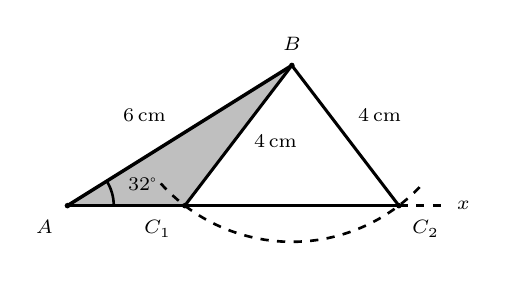
\begin{tikzpicture}[scale=0.56, every node/.style={font=\scriptsize, text=black}]
        \coordinate (A) at (0,0);
        \coordinate (B) at (5.0883, 3.1795);
        \coordinate (C1) at (2.6612, 0);
        \coordinate (C2) at (7.5154, 0);
        \coordinate (Xend) at (8.55, 0);
        \fill[midgray] (A) -- (B) -- (C1) -- cycle;
        \fill[white] (B) -- (C1) -- (C2) -- cycle;
        \draw[black, line width=0.95pt, dashed] (A) -- (Xend) node[right=1pt] {$x$};
        \draw[black, line width=1.25pt] (A) -- (B) node[midway, above left=1pt] {$6\unit{cm}$};
        \draw[black, line width=1.1pt] (B) -- (C1) node[midway, right=2pt, yshift=-2pt] {$4\unit{cm}$};
        \draw[black, line width=1.1pt] (B) -- (C2) node[midway, above right=1pt] {$4\unit{cm}$};
        \draw[black, line width=1.0pt] (A) -- (C2);
        \draw[black, line width=0.95pt, dashed] ($(B)+(-138:4)$) arc (-138:-42:4);
        \draw[black, line width=0.95pt] (1.05,0) arc (0:32:1.05);
        \node at (16:1.78) {$32^\circ$};
        \fill[black] (A) circle (1.8pt) node[below left=1.5pt] {$A$};
        \fill[black] (B) circle (1.8pt) node[above=2pt] {$B$};
        \fill[black] (C1) circle (1.8pt) node[below left=1.5pt] {$C_1$};
        \fill[black] (C2) circle (1.8pt) node[below right=1.5pt] {$C_2$};
      \end{tikzpicture}
      \par\vspace{2pt}\fontsize{8.2pt}{11.8pt}\selectfont
      មុំ $\ang{A}=32^\circ$ \textbf{មិននៅចន្លោះ} $AB$ និង $BC$ $\Rightarrow$ ប៉ោល $4\unit{cm}$ កាត់ $C_1, C_2$ ($\tri{ABC_1}\ncg\tri{ABC_2}$)។
    \end{tcolorbox}
  \end{minipage}
\end{tcolorbox}

\clearpage

% ============================================================================
% ទំព័រទី ៥៖ កាតវិនិច្ឆ័យ «មេដៃបញ្ឆោត» A / B / C / D — E5 Evaluate
% ============================================================================
\pagebanner{សម្ភារៈទី ៥៖ កាតវិនិច្ឆ័យ «មេដៃបញ្ឆោត» \en{A / B / C / D} (ស-ខ្មៅ)}{ទំព័រទី ៥ / ៦ — សកម្មភាព \en{E5 Evaluate} (៦០–៩០ វិនាទី)}

{\fontsize{8.6pt}{12pt}\selectfont
\textbf{វិធីលេងក្នុងថ្នាក់៖} គ្រូលើកកាតម្ដងមួយ $\rightarrow$ សិស្ស \textbf{ចង្អុលខ្យល់ \en{S--A--S}} $\rightarrow$ លើក \textbf{មេដៃឡើង (ពិត)} ឬ \textbf{ខ្វែងដៃ (ខុស/អន្ទាក់)} + បង្ហាញ \textbf{ម្រាម ១–៣} ប្រាប់ទំនុកចិត្ត។}

\vspace{4pt}

% --- ជួរទី ១៖ កាត A & កាត B ---
\noindent
\begin{tcolorbox}[
  enhanced, sharp corners, colback=white, colframe=white,
  borderline={1.0pt}{0pt}{black, dashed},
  width=9.25cm, equal height group=foilrow1, nobeforeafter,
  top=5pt, bottom=5pt, left=6pt, right=6pt
]
  \noindent\colorbox{black}{\textcolor{white}{\Large\textbf{\en{ A }}}}\hspace{0.25cm}{\fontsize{9.5pt}{13pt}\selectfont\textbf{កាត \en{A} ៖ ជ.ម.ជ បង្វិល–ឆ្លុះ $140^\circ$}}\par\vspace{2pt}
  \begin{center}
  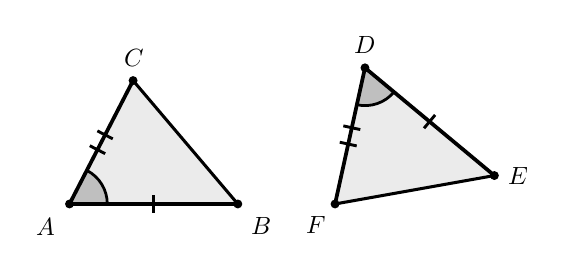
\begin{tikzpicture}[scale=0.95, every node/.style={font=\small, text=black}]
    \coordinate (A) at (0,0);
    \coordinate (B) at (2.25,0);
    \coordinate (C) at (0.85,1.65);
    \fill[panelgray] (A) -- (B) -- (C) -- cycle;
    \pic[draw=black, line width=1.0pt, fill=midgray, angle radius=4.8mm]{angle=B--A--C};
    \draw[black, line width=1.1pt] (B) -- (C);
    \draw[black, line width=1.35pt, tk1] (A) -- (B);
    \draw[black, line width=1.35pt, tk2] (A) -- (C);
    \fill[black] (A) circle (1.7pt) (B) circle (1.7pt) (C) circle (1.7pt);
    \node[below left=1.5pt] at (A) {$A$};
    \node[below right=1.5pt] at (B) {$B$};
    \node[above=1.5pt] at (C) {$C$};
    % ត្រីកោណទី២ (ឆ្លុះ-បង្វិល 140 deg)
    \coordinate (D) at (3.95,1.82);
    \coordinate (E) at (5.68,0.38);
    \coordinate (F) at (3.55,0.00);
    \fill[panelgray] (D) -- (E) -- (F) -- cycle;
    \pic[draw=black, line width=1.0pt, fill=midgray, angle radius=4.8mm]{angle=F--D--E};
    \draw[black, line width=1.1pt] (E) -- (F);
    \draw[black, line width=1.35pt, tk1] (D) -- (E);
    \draw[black, line width=1.35pt, tk2] (D) -- (F);
    \fill[black] (D) circle (1.7pt) (E) circle (1.7pt) (F) circle (1.7pt);
    \node[above=1.5pt] at (D) {$D$};
    \node[right=1.5pt] at (E) {$E$};
    \node[below left=1pt] at (F) {$F$};
  \end{tikzpicture}
  \end{center}
  \vfill
  \begin{tcolorbox}[enhanced, sharp corners, colback=panelgray, colframe=black, boxrule=0.8pt, top=4pt, bottom=4pt, left=5pt, right=5pt]
    \centering\fontsize{9.2pt}{13pt}\selectfont
    \textbf{សំណួរ៖} តើ $\tri{ABC} \cg \tri{DEF}$ ឬទេ?\\[2pt]
    \chkbox\ មេដៃឡើង (ពិត) \hspace{0.5cm} \chkbox\ ខ្វែងដៃ (ខុស/អន្ទាក់)
  \end{tcolorbox}
\end{tcolorbox}%
\hfill
\begin{tcolorbox}[
  enhanced, sharp corners, colback=white, colframe=white,
  borderline={1.0pt}{0pt}{black, dashed},
  width=9.25cm, equal height group=foilrow1, nobeforeafter,
  top=5pt, bottom=5pt, left=6pt, right=6pt
]
  \noindent\colorbox{black}{\textcolor{white}{\Large\textbf{\en{ B }}}}\hspace{0.25cm}{\fontsize{9.5pt}{13pt}\selectfont\textbf{កាត \en{B} ៖ ករណី ជ.ជ.ម មុំក្រៅ}}\par\vspace{2pt}
  \begin{center}
  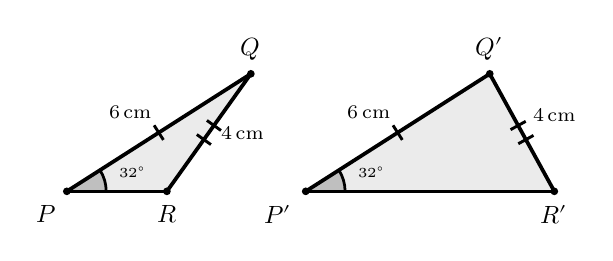
\begin{tikzpicture}[scale=0.82, every node/.style={font=\small, text=black}]
    % ត្រីកោណទី១ (មុំទាលត្រង់ R)
    \coordinate (P) at (0,0);
    \coordinate (R) at (1.55,0);
    \coordinate (Q) at (2.85,1.82);
    \fill[panelgray] (P) -- (R) -- (Q) -- cycle;
    \pic[draw=black, line width=1.0pt, fill=midgray, angle radius=5.0mm]{angle=R--P--Q};
    \draw[black, line width=1.1pt] (P) -- (R);
    \draw[black, line width=1.35pt, tk1] (P) -- (Q);
    \draw[black, line width=1.35pt, tk2] (Q) -- (R);
    \node[font=\tiny] at (16:1.05) {$32^\circ$};
    \node[above left=0.5pt, font=\scriptsize] at ($(P)!0.52!(Q)$) {$6\unit{cm}$};
    \node[right=1pt, font=\scriptsize] at ($(Q)!0.5!(R)$) {$4\unit{cm}$};
    \fill[black] (P) circle (1.7pt) (Q) circle (1.7pt) (R) circle (1.7pt);
    \node[below left=1.5pt] at (P) {$P$};
    \node[above=1.5pt] at (Q) {$Q$};
    \node[below=1.5pt] at (R) {$R$};
    % ត្រីកោណទី២ (មុំស្រួចត្រង់ R')
    \coordinate (Pp) at (3.70,0);
    \coordinate (Rp) at (7.55,0);
    \coordinate (Qp) at (6.55,1.82);
    \fill[panelgray] (Pp) -- (Rp) -- (Qp) -- cycle;
    \pic[draw=black, line width=1.0pt, fill=midgray, angle radius=5.0mm]{angle=Rp--Pp--Qp};
    \draw[black, line width=1.1pt] (Pp) -- (Rp);
    \draw[black, line width=1.35pt, tk1] (Pp) -- (Qp);
    \draw[black, line width=1.35pt, tk2] (Qp) -- (Rp);
    \node[font=\tiny] at ($(Pp)+(16:1.05)$) {$32^\circ$};
    \node[above left=0.5pt, font=\scriptsize] at ($(Pp)!0.52!(Qp)$) {$6\unit{cm}$};
    \node[above right=0.5pt, font=\scriptsize] at ($(Qp)!0.5!(Rp)$) {$4\unit{cm}$};
    \fill[black] (Pp) circle (1.7pt) (Qp) circle (1.7pt) (Rp) circle (1.7pt);
    \node[below left=1.5pt] at (Pp) {$P'$};
    \node[above=1.5pt] at (Qp) {$Q'$};
    \node[below=1.5pt] at (Rp) {$R'$};
  \end{tikzpicture}
  \end{center}
  \vfill
  \begin{tcolorbox}[enhanced, sharp corners, colback=panelgray, colframe=black, boxrule=0.8pt, top=4pt, bottom=4pt, left=5pt, right=5pt]
    \centering\fontsize{9.2pt}{13pt}\selectfont
    \textbf{សំណួរ៖} តើ $\tri{PQR} \cg \tri{P'Q'R'}$ ឬទេ?\\[2pt]
    \chkbox\ មេដៃឡើង (ពិត) \hspace{0.5cm} \chkbox\ ខ្វែងដៃ (ខុស/អន្ទាក់)
  \end{tcolorbox}
\end{tcolorbox}

\vspace{6pt}

% --- ជួរទី ២៖ កាត C & កាត D ---
\noindent
\begin{tcolorbox}[
  enhanced, sharp corners, colback=white, colframe=white,
  borderline={1.0pt}{0pt}{black, dashed},
  width=9.25cm, equal height group=foilrow2, nobeforeafter,
  top=5pt, bottom=5pt, left=6pt, right=6pt
]
  \noindent\colorbox{black}{\textcolor{white}{\Large\textbf{\en{ C }}}}\hspace{0.25cm}{\fontsize{9.5pt}{13pt}\selectfont\textbf{កាត \en{C} ៖ គ្មានសញ្ញា (ស្មាននឹងភ្នែក)}}\par\vspace{2pt}
  \begin{center}
  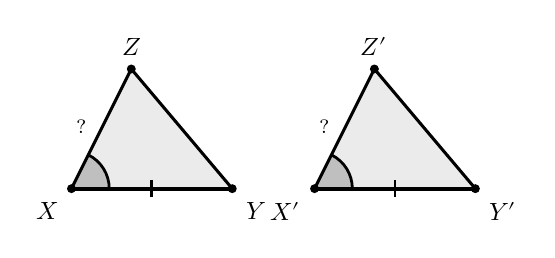
\begin{tikzpicture}[scale=0.95, every node/.style={font=\small, text=black}]
    \coordinate (X) at (0,0);
    \coordinate (Y) at (2.15,0);
    \coordinate (Z) at (0.80,1.60);
    \fill[panelgray] (X) -- (Y) -- (Z) -- cycle;
    \pic[draw=black, line width=1.0pt, fill=midgray, angle radius=4.8mm]{angle=Y--X--Z};
    \draw[black, line width=1.35pt, tk1] (X) -- (Y);
    \draw[black, line width=1.1pt] (X) -- (Z) -- (Y);
    \node[left=2pt, font=\scriptsize] at ($(X)!0.52!(Z)$) {$?$};
    \fill[black] (X) circle (1.7pt) (Y) circle (1.7pt) (Z) circle (1.7pt);
    \node[below left=1.5pt] at (X) {$X$};
    \node[below right=1.5pt] at (Y) {$Y$};
    \node[above=1.5pt] at (Z) {$Z$};
    % ត្រីកោណទី២ មើលទៅស្រដៀងគ្នាប៉ុន្តែជ្រុង XZ vs X'Z' គ្មានសញ្ញា
    \coordinate (Xp) at (3.25,0);
    \coordinate (Yp) at (5.40,0);
    \coordinate (Zp) at (4.05,1.60);
    \fill[panelgray] (Xp) -- (Yp) -- (Zp) -- cycle;
    \pic[draw=black, line width=1.0pt, fill=midgray, angle radius=4.8mm]{angle=Yp--Xp--Zp};
    \draw[black, line width=1.35pt, tk1] (Xp) -- (Yp);
    \draw[black, line width=1.1pt] (Xp) -- (Zp) -- (Yp);
    \node[left=2pt, font=\scriptsize] at ($(Xp)!0.52!(Zp)$) {$?$};
    \fill[black] (Xp) circle (1.7pt) (Yp) circle (1.7pt) (Zp) circle (1.7pt);
    \node[below left=1.5pt] at (Xp) {$X'$};
    \node[below right=1.5pt] at (Yp) {$Y'$};
    \node[above=1.5pt] at (Zp) {$Z'$};
  \end{tikzpicture}
  \end{center}
  \vfill
  \begin{tcolorbox}[enhanced, sharp corners, colback=panelgray, colframe=black, boxrule=0.8pt, top=4pt, bottom=4pt, left=5pt, right=5pt]
    \centering\fontsize{9.0pt}{12.5pt}\selectfont
    \textbf{សំណួរ៖} ហ៊ានថា $\tri{XYZ}\cg\tri{X'Y'Z'}$ (ជ.ម.ជ) ដោយមើលនឹងភ្នែកឬទេ?\\[2pt]
    \chkbox\ មេដៃឡើង (ពិត) \hspace{0.5cm} \chkbox\ ខ្វែងដៃ (ខុស/អន្ទាក់)
  \end{tcolorbox}
\end{tcolorbox}%
\hfill
\begin{tcolorbox}[
  enhanced, sharp corners, colback=white, colframe=white,
  borderline={1.0pt}{0pt}{black, dashed},
  width=9.25cm, equal height group=foilrow2, nobeforeafter,
  top=5pt, bottom=5pt, left=6pt, right=6pt
]
  \noindent\colorbox{black}{\textcolor{white}{\Large\textbf{\en{ D }}}}\hspace{0.25cm}{\fontsize{9.5pt}{13pt}\selectfont\textbf{កាត \en{D} ៖ ម.ម.ម / លំដាប់ខុស $\tri{ABC}\cg\tri{FED}$}}\par\vspace{2pt}
  \begin{center}
  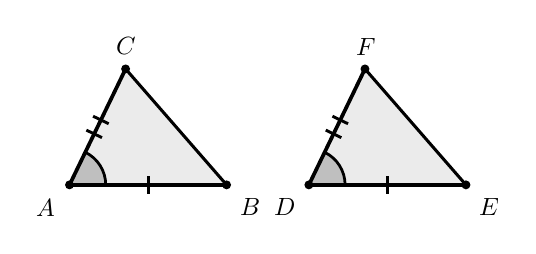
\begin{tikzpicture}[scale=0.95, every node/.style={font=\small, text=black}]
    \coordinate (A) at (0,0);
    \coordinate (B) at (2.10,0);
    \coordinate (C) at (0.75,1.55);
    \fill[panelgray] (A) -- (B) -- (C) -- cycle;
    \pic[draw=black, line width=1.0pt, fill=midgray, angle radius=4.6mm]{angle=B--A--C};
    \draw[black, line width=1.1pt] (B) -- (C);
    \draw[black, line width=1.35pt, tk1] (A) -- (B);
    \draw[black, line width=1.35pt, tk2] (A) -- (C);
    \fill[black] (A) circle (1.7pt) (B) circle (1.7pt) (C) circle (1.7pt);
    \node[below left=1.5pt] at (A) {$A$};
    \node[below right=1.5pt] at (B) {$B$};
    \node[above=1.5pt] at (C) {$C$};
    % ត្រីកោណទី២ មាន D <-> A, E <-> B, F <-> C ប៉ុន្តែប្រធានសរសេរ ΔABC ≅ ΔFED
    \coordinate (D) at (3.20,0);
    \coordinate (E) at (5.30,0);
    \coordinate (F) at (3.95,1.55);
    \fill[panelgray] (D) -- (E) -- (F) -- cycle;
    \pic[draw=black, line width=1.0pt, fill=midgray, angle radius=4.6mm]{angle=E--D--F};
    \draw[black, line width=1.1pt] (E) -- (F);
    \draw[black, line width=1.35pt, tk1] (D) -- (E);
    \draw[black, line width=1.35pt, tk2] (D) -- (F);
    \fill[black] (D) circle (1.7pt) (E) circle (1.7pt) (F) circle (1.7pt);
    \node[below left=1.5pt] at (D) {$D$};
    \node[below right=1.5pt] at (E) {$E$};
    \node[above=1.5pt] at (F) {$F$};
  \end{tikzpicture}
  \end{center}
  {\centering\fontsize{8.1pt}{11pt}\selectfont (ប្រយ័ត្នទាំងលំដាប់កំពូល និងកុំច្រឡំ ម.ម.ម \en{AAA} ថាប៉ុនគ្នា!)\par}
  \vfill
  \begin{tcolorbox}[enhanced, sharp corners, colback=panelgray, colframe=black, boxrule=0.8pt, top=4pt, bottom=4pt, left=5pt, right=5pt]
    \centering\fontsize{9.0pt}{12.5pt}\selectfont
    \textbf{សំណួរ៖} តើការសរសេរ $\tri{ABC} \cg \tri{FED}$ ត្រូវឬខុស?\\[2pt]
    \chkbox\ មេដៃឡើង (ពិត) \hspace{0.5cm} \chkbox\ ខ្វែងដៃ (ខុស/អន្ទាក់)
  \end{tcolorbox}
\end{tcolorbox}

\vspace{7pt}

% --- ខ្សែកាត់ & បន្ទះចម្លើយសម្រាប់គ្រូ (Teacher Mini Answer & Remediation Key) ---
\noindent\scissors\ \dotfill\ \textbf{កាត់ទុកសម្រាប់គ្រូ (\en{Teacher Mini Answer \& Remediation Key})} \dotfill\ \scissors

\vspace{4pt}
\begin{tcolorbox}[
  enhanced, sharp corners, colback=panelgray, colframe=black,
  boxrule=1.0pt, top=4pt, bottom=4pt, left=5pt, right=5pt
]
  \fontsize{7.9pt}{11.2pt}\selectfont
  \renewcommand{\arraystretch}{1.12}
  \begin{tabular}{|L{4.0cm}|L{4.2cm}|L{4.2cm}|L{4.6cm}|}
    \hline
    \cellcolor{headgray}\textbf{កាត \en{A} ៖ មេដៃឡើង (\ding{51})} &
    \cellcolor{headgray}\textbf{កាត \en{B} ៖ ខ្វែងដៃ (\ding{55})} &
    \cellcolor{headgray}\textbf{កាត \en{C} ៖ ខ្វែងដៃ (\ding{55})} &
    \cellcolor{headgray}\textbf{កាត \en{D} ៖ ខ្វែងដៃ (\ding{55})} \\ \hline
    $\tri{ABC}\cg\tri{DEF}$ តាម \textbf{ជ.ម.ជ} ទោះបង្វិល–ឆ្លុះ $140^\circ$។ ចង្អុលខ្យល់ $A\leftrightarrow D$ ផ្ទៀងសញ្ញា \tickone, ធ្នូ, \ticktwo ។ &
    \textbf{អន្ទាក់ ជ.ជ.ម (\en{SSA})}! មុំ $32^\circ$ មិននៅចន្លោះ $6\unit{cm}, 4\unit{cm}$ ($\tri{PQR}$ ទាល $\ncg \tri{P'Q'R'}$ ស្រួច)។ &
    \textbf{គ្មានសញ្ញាជ្រុងទី ២} ($XZ$ vs $X'Z'$)! ហាមស្មានដោយមើលនឹងភ្នែក ត្រូវរកសញ្ញា \cnum{1}--\cnum{3} បញ្ជាក់។ &
    \textbf{ខុសលំដាប់កំពូល!} ត្រូវសរសេរ $\tri{ABC}\cg\tri{DEF}$ ($A\leftrightarrow D$), មិនមែន $\tri{FED}$។ (ម.ម.ម ក៏មិនប៉ុនគ្នា!) \\ \hline
  \end{tabular}
  \par\vspace{3pt}
  \textbf{ត្រួតទំនុកចិត្ត (ម្រាម ១–៣)៖} ១ ម្រាម = ហៅដៃគូចង្អុលជួស \en{S-A-S} ឡើងវិញ \hspace{0.3cm}|\hspace{0.3cm} ២ ម្រាម = ផ្ទៀងធនាគារ \cnum{1}--\cnum{5} \hspace{0.3cm}|\hspace{0.3cm} ៣ ម្រាម = ច្បាស់ ១០០\%
\end{tcolorbox}

\clearpage

% ============================================================================
% ទំព័រទី ៦៖ ប័ណ្ណកិច្ចការផ្ទះ ជំហានទី ៥ (២ ប័ណ្ណក្នុង ១ ទំព័រ A4)
% ============================================================================
\pagebanner{សម្ភារៈទី ៦៖ ប័ណ្ណកិច្ចការផ្ទះ ជំហានទី ៥ — ២ ប័ណ្ណក្នុង ១ ទំព័រ \en{A4}}{ទំព័រទី ៦ / ៦ — ជំហានទី ៥ (កាត់ចែកតាម \scissors)}

% និយមន័យម៉ាក្រូប័ណ្ណកិច្ចការផ្ទះ (២ ប័ណ្ណដូចគ្នាទាំងស្រុង word-for-word ពី LS_Plan_SAS.tex)
\newcommand{\hwslip}[1]{%
\begin{tcolorbox}[
  enhanced, sharp corners, colback=white, colframe=black,
  boxrule=1.1pt, top=5pt, bottom=5pt, left=6pt, right=6pt
]
  \begin{tcolorbox}[
    enhanced, sharp corners, colback=headgray, colframe=black,
    boxrule=0.7pt, top=2.5pt, bottom=2.5pt, left=5pt, right=5pt, after skip=5pt
  ]
    \fontsize{8.8pt}{12pt}\selectfont
    \textbf{ប័ណ្ណកិច្ចការផ្ទះ (#1) — អនុវិទ្យាល័យព្រះក្រសាំង | គណិតវិទ្យា ថ្នាក់ទី៨} \hfill \textbf{មេរៀនទី១២៖ ១.២.២ ករណី ជ.ម.ជ (\en{SAS})}\\[2pt]
    ឈ្មោះសិស្ស៖ $\underline{\hspace{4.8cm}}$ \hspace{0.3cm} ថ្នាក់ទី៖ $\underline{\hspace{1.4cm}}$ \hspace{0.3cm} កាលបរិច្ឆេទ៖ $\underline{\hspace{3.0cm}}$
  \end{tcolorbox}

  \noindent
  \begin{minipage}[c]{12.2cm}
    \fontsize{9.1pt}{13.6pt}\selectfont
    {\muol កិច្ចការផ្ទះ} \textbf{៖} គេមាន $\tri{ABC}$ ($AB = AC$), កន្លះបន្ទាត់ពុះ $AD$ នៃ $\ang{BAC}$ ($D \in BC$), និង $E \in AD$ ($E \neq A, D$) ។\\[4pt]
    \hspace*{0.2cm}\textbf{ក.} បង្ហាញថា $\tri{ABD} \cg \tri{ACD}$ រួចទាញថា $DB = DC$ និង $\ang{ADB} = \ang{ADC}$ ។\\[2pt]
    \hspace*{0.2cm}\textbf{ខ.} ស្រាយបញ្ជាក់ថា $\tri{BDE} \cg \tri{CDE}$ រួចទាញថា $EB = EC$ និង $\ang{DBE} = \ang{DCE}$ ។\\[5pt]
    {\fontsize{8.3pt}{11.8pt}\selectfont
    \textbf{តម្រុយធនាគារអំណះអំណាង \cnum{1}--\cnum{5}៖} \cnum{1} បម្រាប់ ($AB=AC$) | \cnum{2} ពុះមុំ | \cnum{3} ជ្រុងរួម ($AD=AD$, $DE=DE$) | \cnum{4} ជ.ម.ជ | \cnum{5} ធាតុត្រូវគ្នា។\\[2pt]
    \textbf{គ្រោងផែនការ៖} (ក) \cnum{1} $AB=AC$, \cnum{2} $\ang{BAD}=\ang{CAD}$, \cnum{3} $AD=AD$ $\Rightarrow$ \cnum{4} $\Rightarrow$ \cnum{5} \hspace{0.15cm}|\hspace{0.15cm} (ខ) វិបាក (ក) + \cnum{3} $DE=DE$ $\Rightarrow$ \cnum{4} $\Rightarrow$ \cnum{5}}
  \end{minipage}%
  \hfill
  \begin{minipage}[c]{5.9cm}
    \centering
    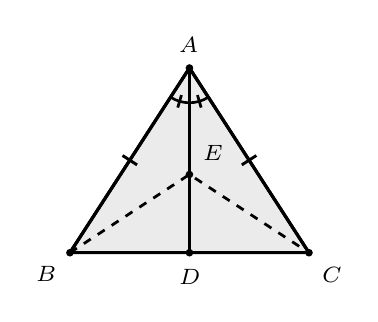
\begin{tikzpicture}[scale=0.92, every node/.style={font=\footnotesize, text=black}]
      \coordinate (A) at (0, 2.55);
      \coordinate (B) at (-1.65, 0);
      \coordinate (C) at (1.65, 0);
      \coordinate (D) at (0, 0);
      \coordinate (E) at (0, 1.08);
      \fill[panelgray] (A) -- (B) -- (C) -- cycle;
      \draw[black, line width=1.1pt] (A) -- (B) -- (C) -- cycle;
      \draw[black, line width=1.3pt] (A) -- (D);
      \draw[black, line width=1.0pt, dashed] (B) -- (E) -- (C);
      \draw[black, line width=1.15pt, tk1] (A) -- (B);
      \draw[black, line width=1.15pt, tk1] (A) -- (C);
      \draw[black, line width=0.95pt] ($(A)+(-122.90:0.48)$) arc (-122.90:-57.10:0.48);
      \draw[black, line width=1.0pt] ($(A)+(-106.45:0.39)$) -- ($(A)+(-106.45:0.57)$);
      \draw[black, line width=1.0pt] ($(A)+(-73.55:0.39)$) -- ($(A)+(-73.55:0.57)$);
      \fill[black] (A) circle (1.5pt) node[above=2pt] {$A$};
      \fill[black] (B) circle (1.5pt) node[below left=1.5pt] {$B$};
      \fill[black] (C) circle (1.5pt) node[below right=1.5pt] {$C$};
      \fill[black] (E) circle (1.5pt) node[above right=1.5pt] {$E$};
      \fill[black] (D) circle (1.5pt) node[below=2.5pt] {$D$};
    \end{tikzpicture}
  \end{minipage}

  \vspace{5pt}
  \begin{tcolorbox}[
    enhanced, sharp corners, colback=panelgray, colframe=black,
    boxrule=0.8pt, top=3.5pt, bottom=3.5pt, left=5pt, right=5pt
  ]
    \fontsize{8.3pt}{12.0pt}\selectfont
    \textbf{បញ្ជីផ្ទៀងផ្ទាត់ខ្លួនឯងរបស់សិស្ស (\en{3-Box Student Self-Check List})៖}\\[2pt]
    \chkbox\ \textbf{១.} ខ្ញុំបានចង្អុលគូសសញ្ញា \tickone, \ticktwo\ និងព័ទ្ធកំពូលរួមលើរូប ព្រមទាំងដាក់លេខ \cnum{1}--\cnum{5} គ្រប់បន្ទាត់ (រួមទាំង \cnum{3} ជ្រុងរួម $AD=AD$ និង $DE=DE$)។\\[1.5pt]
    \chkbox\ \textbf{២.} ខ្ញុំបានផ្ទៀងលំដាប់កំពូល $A\to B\to D$ ទល់ $A\to C\to D$ (សំណួរ ក) និង $B\to D\to E$ ទល់ $C\to D\to E$ (សំណួរ ខ) ។\\[1.5pt]
    \chkbox\ \textbf{៣.} ខ្ញុំបានប្រើសញ្ញា $=$ សម្រាប់ប្រវែង/រង្វាស់មុំ និង $\cg$ សម្រាប់ត្រីកោណប៉ុនគ្នា ព្រមទាំងភ្ជាប់វិបាក (ក) ទៅ (ខ) ត្រឹមត្រូវ។
  \end{tcolorbox}
\end{tcolorbox}%
}

\hwslip{ប័ណ្ណទី ១}

\vspace{7pt}
\noindent\scissors\ \dotfill\ \textbf{កាត់តាមស្នាមចុចចែកជា ២ ប័ណ្ណ (\en{Cut Along Dashed Line})} \dotfill\ \scissors
\vspace{7pt}

\hwslip{ប័ណ្ណទី ២}

\end{document}
